
\chapter{\IfLanguageName{dutch}{Praktische uitvoering van ANPR}{Implementation of ANPR at UGent}}
\label{ch:praktischeUitvoering}
In dit hoofdstuk wordt er onderzocht of nummerplaatdetectie degelijke resultaten kan behalen op de Campus Sterre en Campus Coupure van UGent. Hiervoor zullen handmatig foto's genomen worden van wagens die de parking verlaten a.d.h.v. een testopstelling van een Raspberry Pi met een Pi-NoIR camera. Vervolgens worden deze foto's verwerkt met OpenALPR en zullen deze resultaten vergeleken worden met de correcte resultaten. Op deze manier wordt de nauwkeurigheid van de nummerplaatdetectie per uitgang bepaalt en kan een conclusie getrokken worden of dit wel degelijk een haalbare technologie is.

\section{Opstelling}
In dit onderdeel wordt de opstelling en configuratie van de camera's uitgelegd a.d.h.v. de informatie verzameld in Hoofdstuk \ref{ch:maatregelenanpr}.

\subsection{Camera}
Als camera wordt gebruik gemaakt van de PiNoIR-Cam. Deze camera is een uitbreiding voor de Raspberry-PI dat geen infrarood filtering heeft staan. Bij andere camera's wordt infrarood licht uit afbeeldingen gefilterd aangezien dit een ongewenste verkleuring aan de afbeeldingen geeft. Door dit licht toch door te laten wordt het mogelijk om 's nachts foto's te nemen.

\paragraph{Cameraplaatsing}
De plaatsing van de camera's dient zo kostenefficiënt mogelijk te zijn, waardoor liefst geen aparte paal voor de ANPR-camera wordt bijgeplaatst. Hierdoor is eerste keuze om de ANPR-camera te monteren de metalen constructie van de hefboom zelf. De camera is hier zo hoog mogelijk aangehangen zodat deze het minst interferentie heeft van de koplampen van de auto's.

\begin{figure}[h!]
	\centering
	\includegraphics[width=\linewidth]{img/uitgang-coupure.jpg}
	\caption{Uitgang met tokens aan UGent campus Coupure}
\end{figure}

\subsection{Opstelling}
Om de foto's te verkrijgen is gebruik gemaakt van de Raspberry Pi met de PiNoIR camera, deze is op de juiste hoogte van de paal tijdelijk vastgezet worden tezamen met een powerbank. De Raspberry Pi is geconnecteerd met een GSM die als hotspot ingesteld staat, waarop met een SSH verbinding het commando kan worden uitgevoerd om foto's te nemen. Deze foto's worden vervolgens allemaal verzameld en verwerkt.

Figuur \ref{Opstelling} toont de gemaakte opstelling. Deze bevat De Raspberry Pi, de Pi-Cam en een powerbank met een capaciteit van 700mAh.
\begin{figure}[h]
	\centering
	\includegraphics[width=0.5\linewidth]{img/camera.jpg}
	\caption{Opstelling Raspberry Pi met PiCam.}
	\label{Opstelling}
\end{figure}

\section{Verzamelen van de gegevens}
De verzamelde gegevens horen correct te zijn en representatief voor een automatisch geïmplementeerd systeem. Alle uitgevoerde stappen om de gegevens te bekomen zijn in dit onderdeel beschreven tezamen met hun motivaties.

\subsection{Nemen van de foto's}
Het nemen van de foto's is een fysiek onderdeel van dit onderzoek en werd uitgevoerd op de volgende locaties:
\begin{itemize}
	\item Campus Coupure - Uitgang Coupure Links
	\item Campus Coupure - Uitgang Kruisboogstraat
	\item Campus Sterre - Uitgang De Pintelaan
	\item Campus Sterre - Uitgang Galglaan
\end{itemize}

Deze foto's werden gemaakt met de PiNoIR camera verbonden aan de Raspberry Pi m.b.v. het raspistill commando. Per auto die de parking verlaat worden er a.d.h.v. een handmatige trigger 6 foto's gemaakt in een burst van 3 seconden met 500 ms per foto. Dit aan de hand van het raspistill commando:  
\begin{lstlisting}[language=Bash, breaklines=true]
#!/bin/bash

# -t : De timeout waarover foto's genomen worden
# -bm : Gebruik de camera in burst mode, hierdoor moet de camera niet telkens opnieuw focussen tussen iedere genomen foto
# -tl : Tijd tussen iedere foto in burst mode
# --width --height : De resolutie van de bekomen foto's
# --nopreview : schakel de preview uit aangezien er geen monitor verbonden is
raspistill -t 3000 -bm -tl 500 --width 1280 --height 720 --nopreview
-o `date +%d%m%Y_%H%M%S`%04d.jpg
\end{lstlisting}

\subsubsection{Triggering van de camera}
De camera zelf werd in dit onderzoek handmatig getriggerd aangezien een implementatie opstellen voor automatische triggering niet paste binnen het tijdsschema van dit onderzoek.

In een werkelijke implementatie zou deze triggering mogelijk zijn a.d.h.v. software dat de beelden van de Raspberry Pi bekijkt en hierop bewegingsdetectie uitvoert. Een voorbeeld hiervan is de 'motion' package die hiervoor een open-source implementatie geeft.

\subsection{Tijdstippen van de genomen foto's}
In tabel \ref{tab:fototijdstippen} zijn alle momenten genoteerd dat er fysiek foto's verzameld werden. Deze zijn telkens verworven in de vroege namiddag aangezien er op deze momenten nog steeds daglicht is en mensen beginnen te vertrekken van de Campussen. Enkel op de Coupure Links is er later geprobeerd data te verzamelen omdat er overdag bijna geen auto's vertrokken.
\begin{table}[h!]
\centering
\begin{tabular}{l|l|l|l|l}
	Datum 		& Begin & Eind	& Locatie	& Aantal foto's \\ \hline
	06/11/2019	& 11u45 & 12u46	& Campus Coupure - Uitgang Kruisboogstraat	& 48	\\
	08/11/2019	& 12u15 & 12u29	& Campus Sterre - Uitgang Galglaan	& 17	\\
	08/11/2019	& 12u52 & 13u41	& Campus Sterre - Uitgang De Pintelaan	& 38	\\
	13/11/2019	& 11u36 & 12u08	& Campus Sterre - Uitgang De Pintelaan	& 50	\\
	13/11/2019	& 12u29 & 12u42	& Campus Sterre - Uitgang Galglaan	& 9	\\
	13/11/2019	& 13u48 & 14u35	& Campus Coupure - Uitgang Coupure Links	& 5	\\
	14/11/2019	& 18u05 & 18u55	& Campus Coupure - Uitgang Coupure Links	& 3	\\
	21/11/2019	& 14u08 & 15u11	& Campus Sterre - Uitgang De Pintelaan	& 35	\\
	21/11/2019	& 15u58 & 16u22	& Campus Sterre - Uitgang Galglaan	& 36	\\
	27/11/2019	& 13u42 & 15u03	& Campus Sterre - Uitgang De Pintelaan	& 75	\\
	29/11/2019	& 12u04 & 12u35	& Campus Coupure - Uitgang Kruisboogstraat	& 20	\\
	11/12/2019	& 13u42 & 15u12	& Campus Sterre - Uitgang De Pintelaan	& 64	\\
\end{tabular}
\caption{Tijdstippen wanneer de verwerkte foto's bekomen zijn.}
\label{tab:fototijdstippen}
\end{table}

%Zo bekomen we volgende aantallen van foto's per uitgang:
%\begin{table}[h]
%	\centering
%	\begin{tabular}{l|l}
%		Uitgang	& Aantal foto's \\ \hline
%		Campus Coupure - Uitgang Kruisboogstraat	& 53\\
%		Campus Coupure - Uigang Coupure Links	& 5\\
%		Campus Sterre - Uitgang Galglaan	& 32\\
%		Campus Sterre - Uitgang De Pintelaan, camerahoek rechts	& 38\\
%		Campus Sterre - Uitgang De Pintelaan, camerahoek links	& 50\\
%	\end{tabular}
%\end{table}

\subsection{Incorrecte foto's}
Foto's die te laat of te vroeg werden genomen worden weggelaten. Enkele voorbeelden hiervan zijn te zien in Figuur \ref{fig:badpics}. Vervolgens wordt er per auto maar 1 foto bijgehouden per afstand. Indien er maar 1 afstand aanwezig is op de foto's, wordt deze reeks niet gezien als representatief en zullen de auto's niet verwerkt worden.

\begin{figure}[h!]
	\centering
	\begin{subfigure}[b]{0.45\linewidth}
		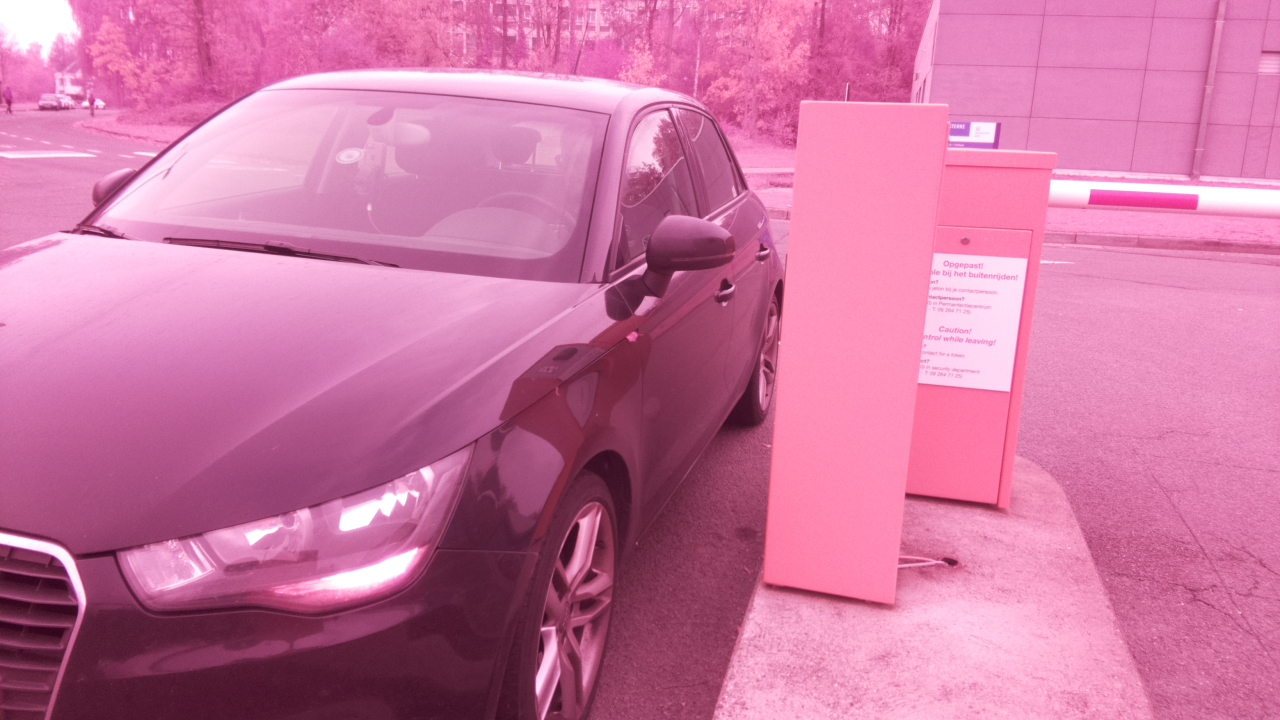
\includegraphics[width=\linewidth]{img/slecht/close.jpg}
		\caption{Auto op een onredelijk dichte afstand.}
	\end{subfigure}
	\begin{subfigure}[b]{0.45\linewidth}
		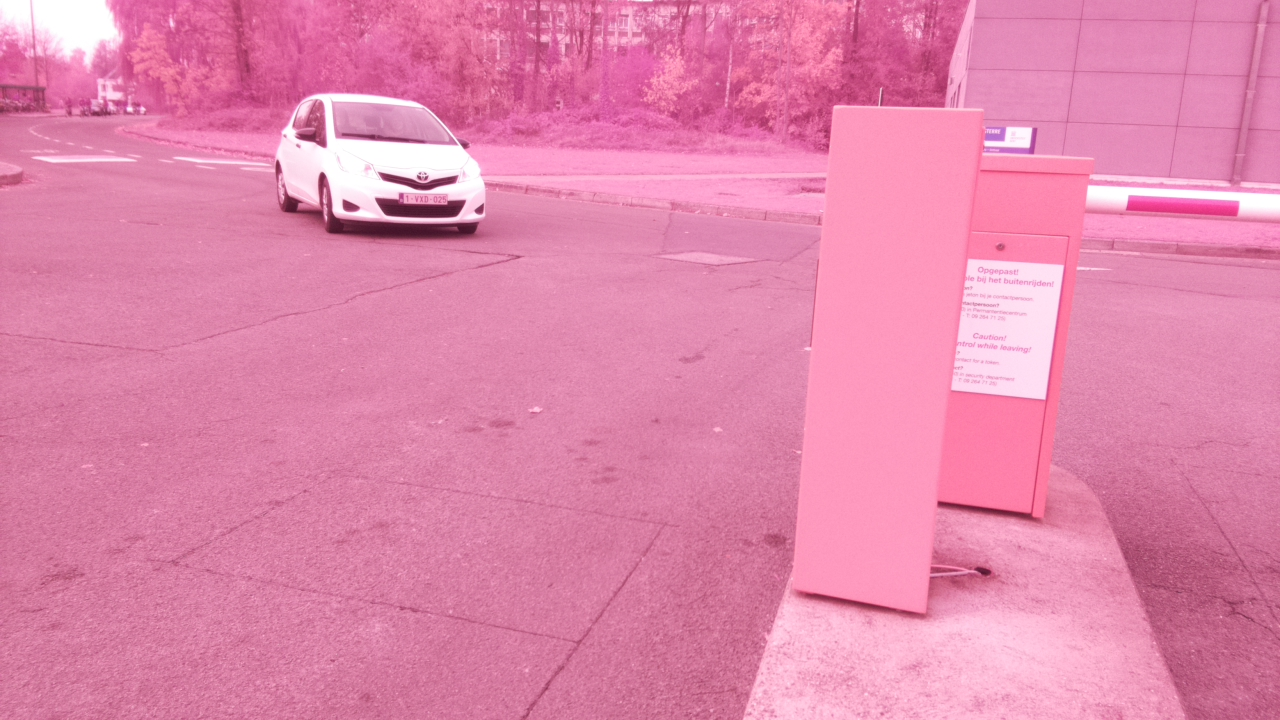
\includegraphics[width=\linewidth]{img/slecht/far.jpg}
		\caption{Auto op een onredelijk verre afstand.}
	\end{subfigure}
	\begin{subfigure}[b]{0.45\linewidth}
		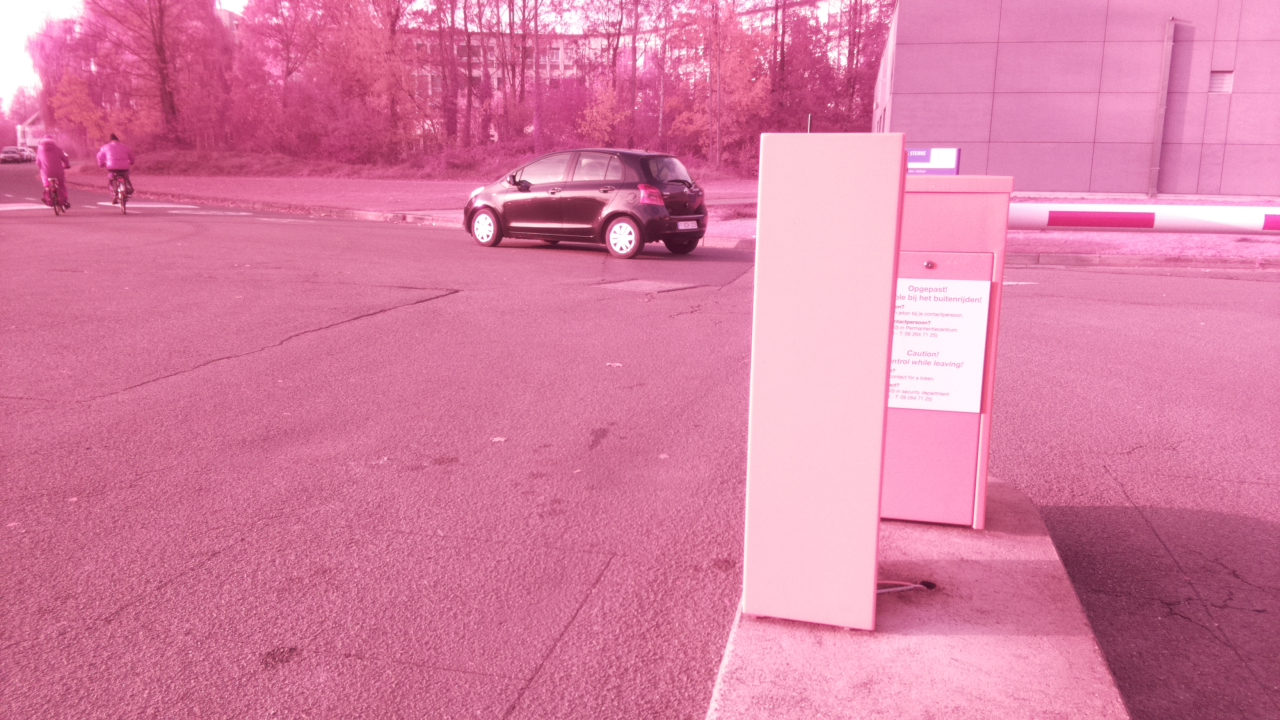
\includegraphics[width=\linewidth]{img/slecht/anderekant.jpg}
		\caption{Auto die de parking niet verlaat.}
	\end{subfigure}
	\caption{Types van foto's die niet werden opgenomen in het onderzoek.}
	\label{fig:badpics}
\end{figure}


In sommige gevallen zijn de foto's allemaal van een veel te verre afstand genomen, dit is niet representatief aangezien een motion detection systeem foto's over een korte afstand kan nemen. In het geval van Figuur \ref{fig:onlyfar} zijn alle afbeeldingen op een verre afstand genomen. Een motion detection systeem zou in dit geval ook foto's genomen kunnen hebben op een dichtere afstand, hierdoor is deze reeks foto's niet representatief en zal ook niet opgenomen worden in het onderzoek.
\begin{figure}[h!]
	\centering
	\begin{subfigure}[b]{0.45\linewidth}
		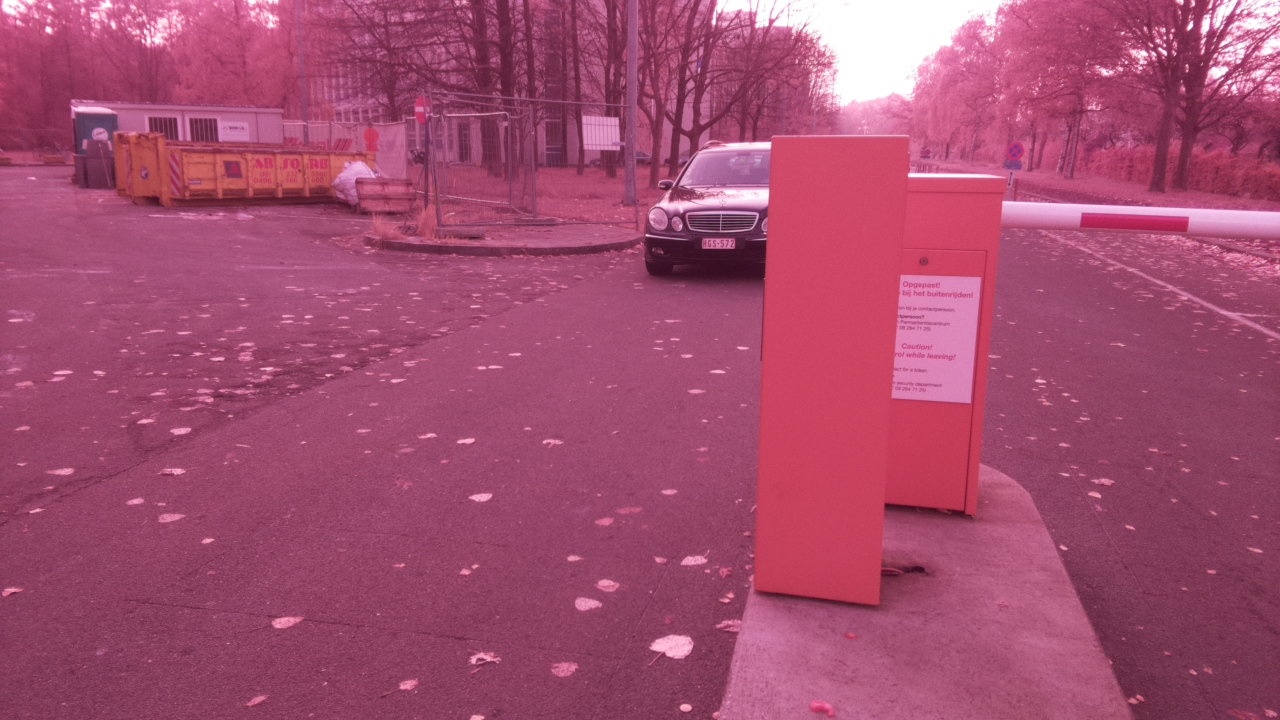
\includegraphics[width=\linewidth]{img/slecht/onlyfar1.jpg}
	\end{subfigure}
	\begin{subfigure}[b]{0.45\linewidth}
		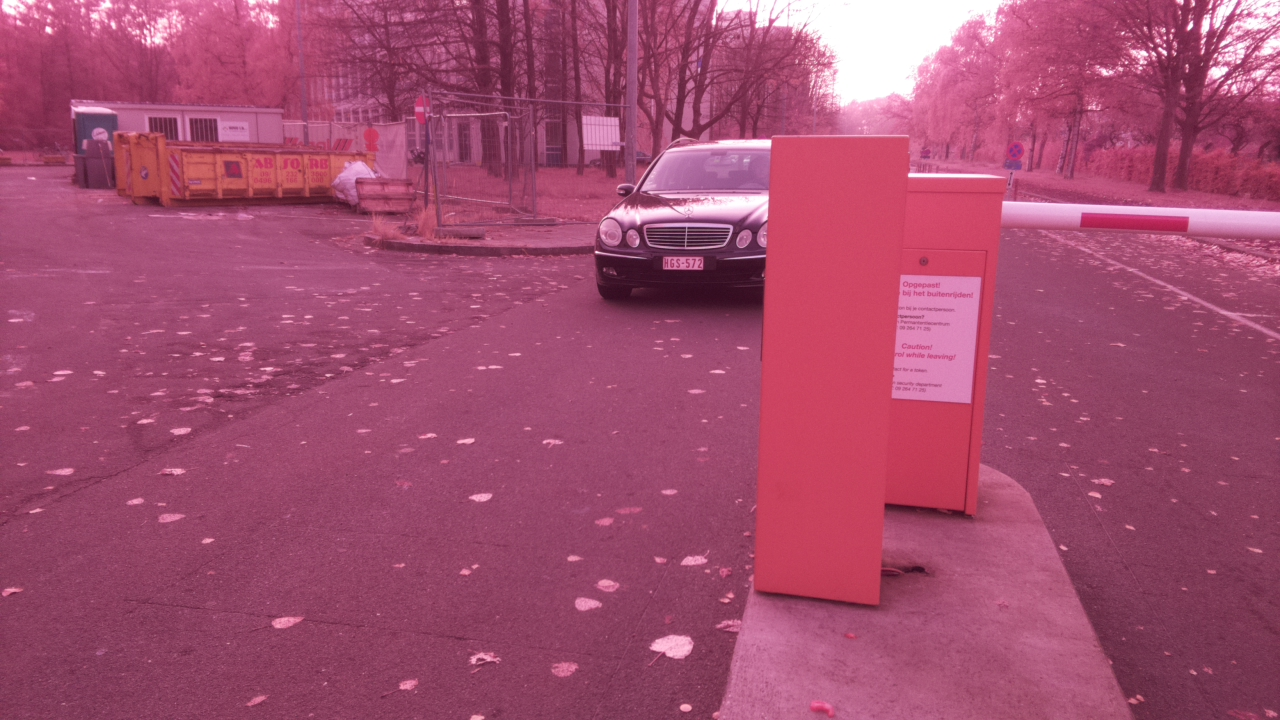
\includegraphics[width=\linewidth]{img/slecht/onlyfar2.jpg}
	\end{subfigure}
	\begin{subfigure}[b]{0.45\linewidth}
		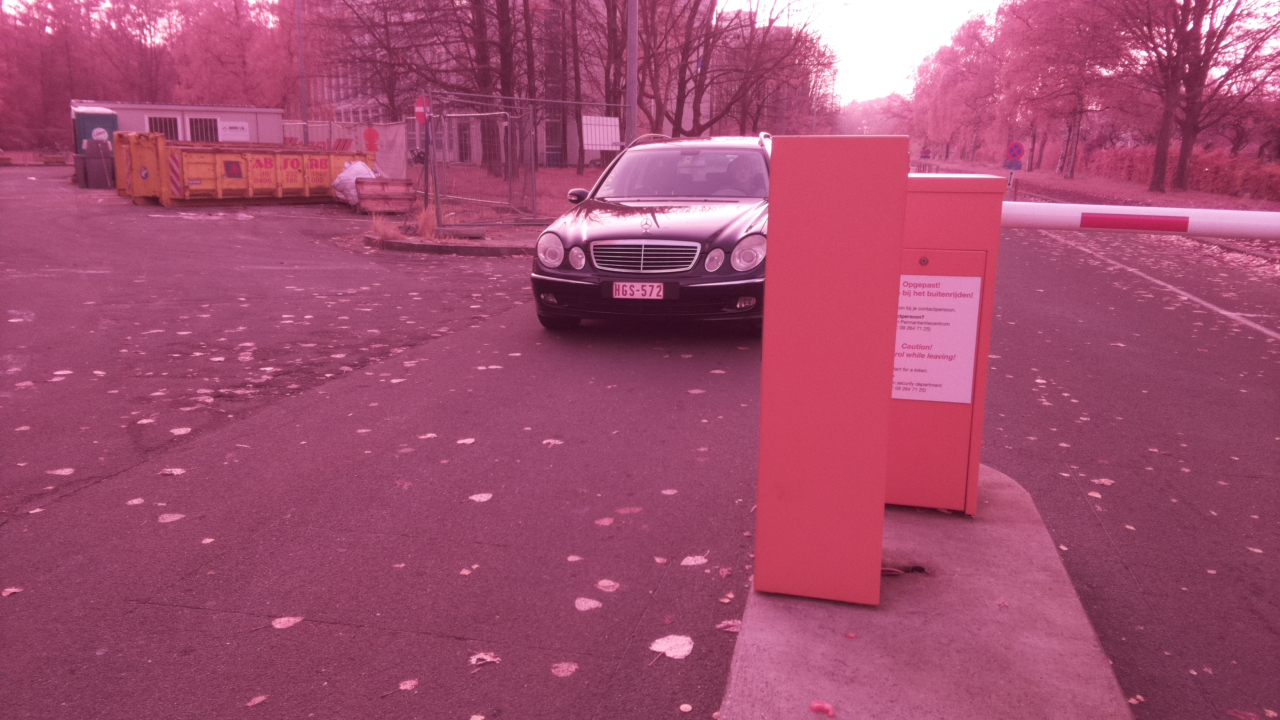
\includegraphics[width=\linewidth]{img/slecht/onlyfar3.jpg}
	\end{subfigure}
	\caption{Foto's die op een te verre afstand genomen zijn en dus niet representatief zijn.}
	\label{fig:onlyfar}
\end{figure}

\section{Verwerking van gegevens}

Nadat de foto's van een uitgang verzameld zijn, werd op iedere foto nummerplaatdetectie uitgevoerd m.b.v. OpenALPR. Het resultaat van deze detectie werd opgeslagen in een JSON bestand naast de corresponderende afbeelding. Hiervoor werd de volgende bash code gebruikt:

\begin{lstlisting}[language=Bash, breaklines=true]
#!/bin/bash

FILES=$(ls -tr *.jpg)
for fullname in $FILES
do
fname="${fullname%.*}"
alpr -p be -c eu --config alpr.config -j $fullname | jq '.' > "${fname}.json"
echo "processed file ${fname}.json" 
done
\end{lstlisting}

Vervolgens werd alle data van de afbeeldingen verzameld in een algemeen CSV bestand, tezamen met de bekomen nummerplaten van OpenALPR.
\begin{itemize}
	\item \textbf{identifier:} Unieke identifier per auto.
	\item \textbf{file:} De bestandsnaam van de foto.
	\item \textbf{license\_plate:} De 'correcte' nummerplaat, handmatig uit de foto gehaald.
	\item \textbf{result:} De nummerplaat gedetecteerd door OpenALPR.
	\item \textbf{distance:} De afstand van de camera, bestaat uit drie velden, "close", "medium"\ en "far". Close betekent een afstand onder de 3 meter, medium tussen 3 en 5 meter en far betekent verder dan 5 meter.
	\item \textbf{lighting:} De belichting van de nummerplaten, bestaat uit 2 velden, "bright"\ en "very\_bright". Bright betekent dat de nummerplaat duidelijk leesbaar is voor mensen onder normaal daglicht. very\_bright betekent dat deze niet onmiddelijk leesbaar is.
	\item \textbf{location:} De uitgang waar de foto is genomen, bestaat uit "coupure-kruisboogstraat", "coupure-coupurelinks", "sterre-galglaan"\ en "sterre-depintelaan".
\end{itemize}

Ten laatste zijn deze resultaten verwerkt in de statistische taal 'R'. De code voor deze bewerkingen zijn te vinden in bijlage \ref{ch:bijlageperfoto} en bijlage \ref{ch:bijlageperauto}.

\subsection{Kalibratie van de afbeeldingen}
Origineel waren alle resultaten van de nummerplaatdetectie aan de zeer lage kant, aangezien de afbeeldingen nog niet gekalibreerd waren. Maar met de tools beschreven in onderdeel \ref{alprcalib}, was het mogelijk om een algemene transformatie op de afbeeldingen uit te voeren.
\begin{figure}[h!]
	\centering
	\begin{subfigure}[b]{0.4\linewidth}
		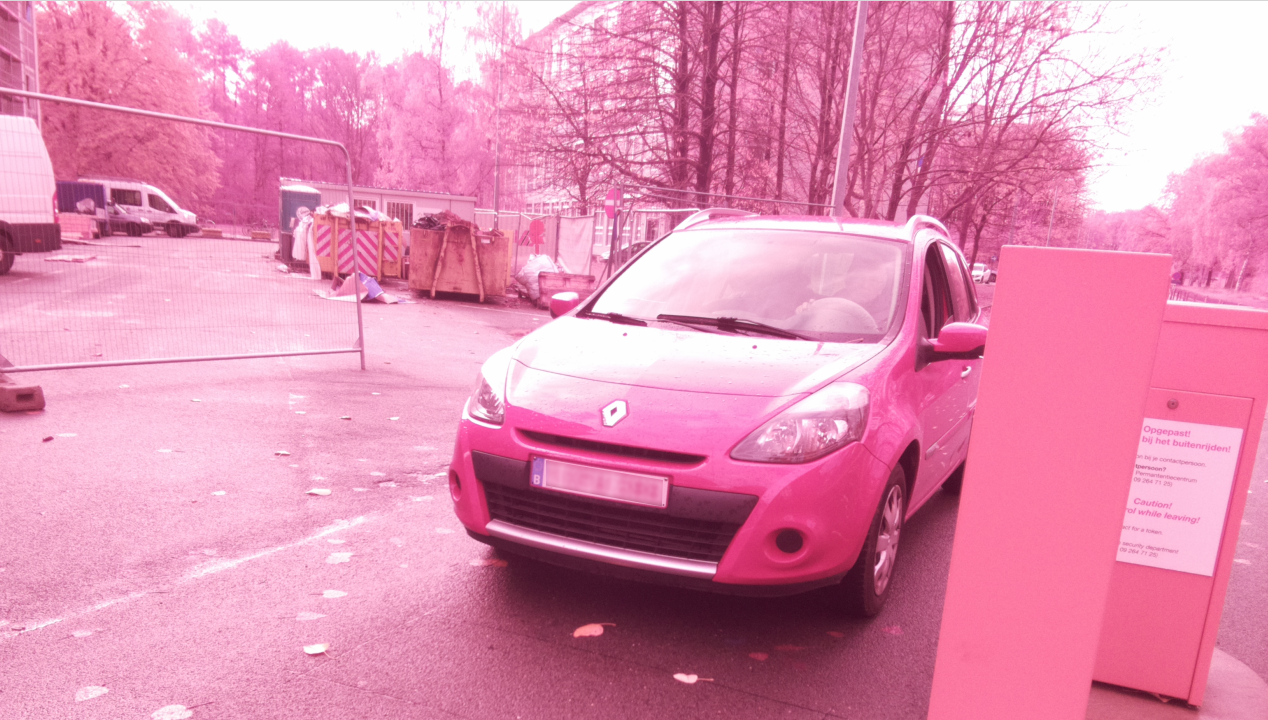
\includegraphics[width=\linewidth]{img/calibration/pre-calibrate.png}
		\caption{Niet-gekalibreerde afbeelding}
	\end{subfigure}
	\begin{subfigure}[b]{0.4\linewidth}
		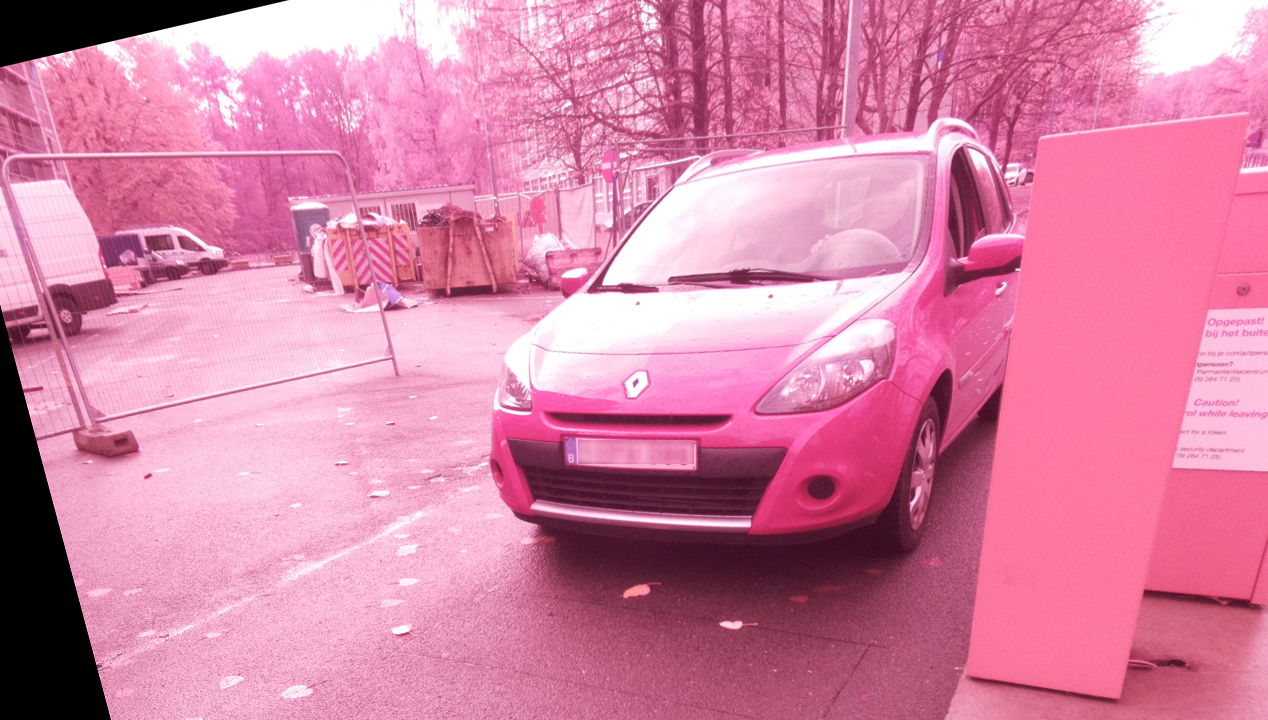
\includegraphics[width=\linewidth]{img/calibration/calibrate-cut.png}
		\caption{Gekalibreerde afbeelding}
	\end{subfigure}
	\label{fig:calibration}
	\caption{Calibratie van afbeeldingen met behulp van openalpr-utils-calibrate.}
\end{figure}

Het verschil in de bekomen resultaten is duidelijk merkbaar. In tabel \ref{tab:kalibratiealpr} worden de resultaten per foto vergeleken waarbij wel gekalibreerd en niet-gekalibreerd is. De resultaten stijgen van een 41.9\% naar een 79.0\%. Kalibratie is dus wellicht een noodzakelijk onderdeel van een geslaagde implementatie.
\begin{table}[h!]
	\centering
	\begin{tabular}{l|l|l|l|l}
		 		& Incorrect & Correct & Totaal & Ratio	\\ \hline
		Niet-gekalibreerd	& 36 & 26 & 62 & 41.9\%	\\
		Gekalibreerd	& 13 & 49 & 62 & 79.0\%\\
	\end{tabular}
\caption{Verschil in nauwkeurigheid per foto door de kalibratie van OpenALPR.}
\label{tab:kalibratiealpr}
\end{table}

\subsection{Patroon matching van nummerplaten}
Nummerplaten kunnen soms foutief gedetecteerd worden door letters en nummers die op elkaar lijken. Zo is er maar een klein verschil tussen de O, 0 en Q. 
Hierdoor kan het zijn dat een nummerplaat zoals 1-NOP-123 gelezen wordt als 1-N0P-123. In de gevallen dat deze de structuur van de reeksen tekens in de nummerplaten verhinderen, kunnen deze gemakkelijk opgelost worden door gebruik van OpenALPR's patroon matching.

Wat patroon matching doet is zoals de naam zegt; het controleren of een bekomen nummerplaat voldoet aan een bepaald patroon. In België en Nederland zijn deze sinds 2010 een 1 met 3 letters en 3 cijfers.

\section{Resultaten}

\subsection{Campus Sterre - Uitgang Galglaan}

De uitgang aan de Galglaan is één van de twee uitgangen op de campus Sterre. De uitgang ligt naast de straat Galglaan en heeft twee inrijrichtingen. Deze locatie is aangeduid in figuur \ref{fig:satteliet-galglaan}.
\begin{figure}[h!]
	\centering
	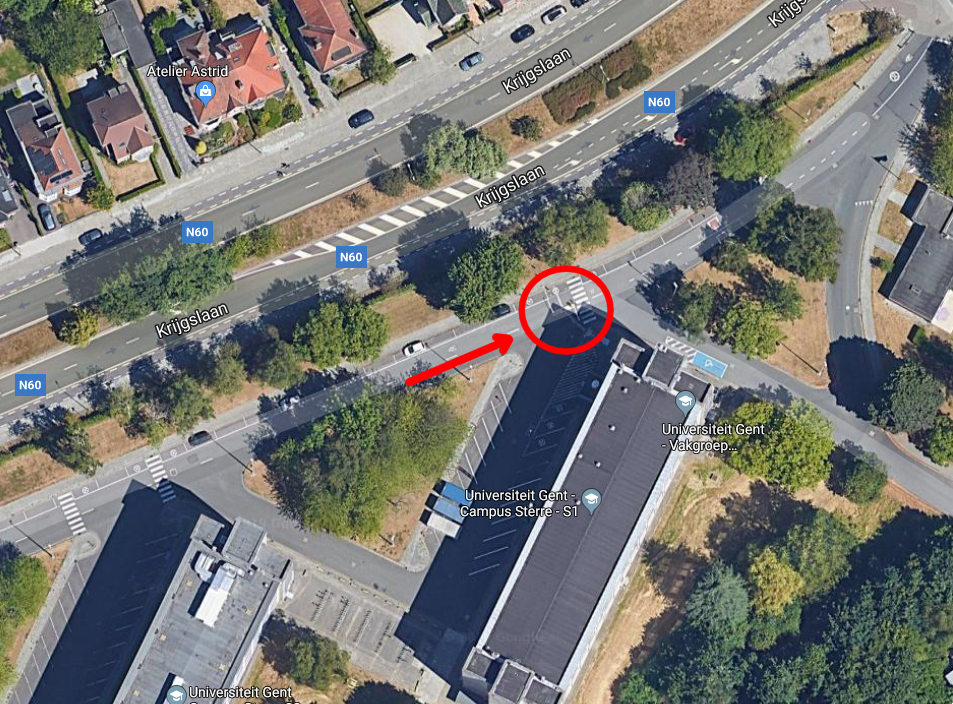
\includegraphics[width=0.8\linewidth]{img/res-galglaan/satteliet-galglaan.png}
	\caption{Satellietafbeelding van de Campus Sterre - Uitgang Galglaan. De uitgang zelf is aangeduid met een rode cirkel. De uitrijrichting met een rode pijl. \autocite{ugent2019google}}
	\label{fig:satteliet-galglaan}
	\centering
	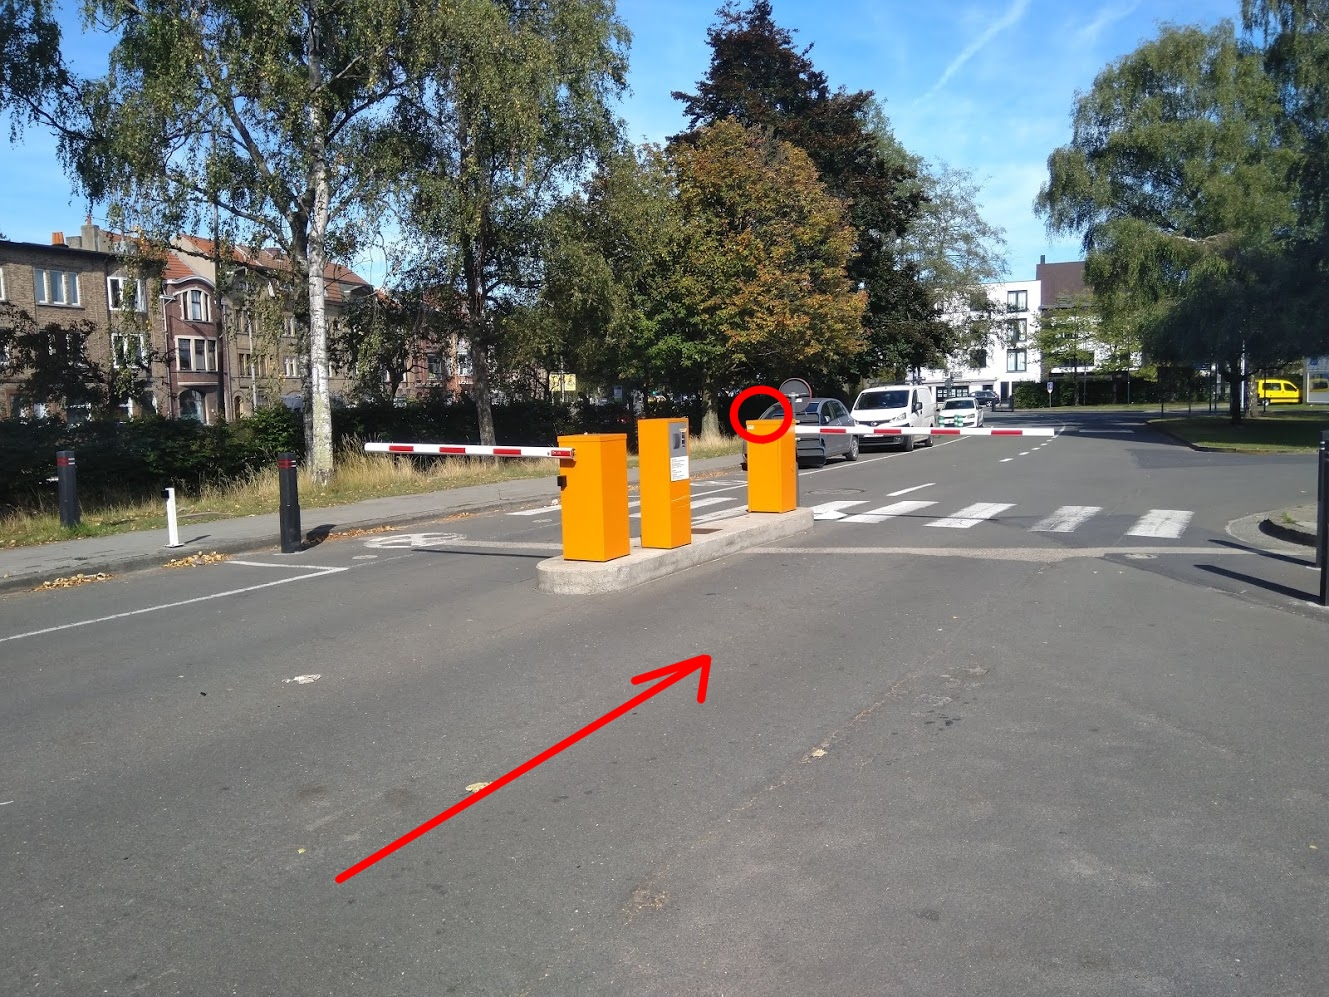
\includegraphics[width=0.8\linewidth]{img/res-galglaan/galg.jpg}
	\caption{Close-up van de uitgang aan Campus Sterre - Uitgang Galglaan. De cameralocatie is aangeduid met een rode cirkel en de uitrijrichting met een rode pijl.}
	\label{fig:galglaan}
\end{figure}

Aan de hand van de informatie bekomen in hoofdstuk \ref{ch:maatregelenanpr}, werd er besloten om de camera op de metalen constructie van de hefboom te plaatsen. Deze is te zien in figuur \ref{fig:galglaan} en is gekozen op basis van de volgende standpunten:
\begin{itemize}
	\item De hoogte van de metalen constructie is hoog genoeg om direct licht van koplampen te verhelpen.
	\item Vanuit deze locatie is een grote afstand van de rijbaan zichtbaar van aankomende voertuigen. Dit geeft het systeem een grotere kans om een auto te identificeren.
	\item De camera op de metalen constructie monteren is een voordeel op vlak van implementatiekosten. Bekabeling is reeds aanwezig in de kast en geen extra paal moet geplaatst worden om de camera te monteren.
\end{itemize}

\paragraph{Resultaat}
Met deze gekozen cameraplaatsing zijn vervolgens 23 verschillende voertuigen verwerkt en zijn de volgende resultaten bekomen:
\begin{table}[h!]
	\centering
	\begin{tabular}{l|l|l|l|l}
\textbf{ANPR nauwkeurigheid: Galglaan} & Incorrect & Correct & Totaal & Ratio	\\ \hline
Per individuele foto 	& 13 & 49	& 62	& 79.0\%\\
Per auto				& 1 & 22	& 23 	& 95.7\%\\
\end{tabular}
\caption{Resultaten van OpenALPR aan Campus Sterre - Uitgang Galglaan.}
\label{tab:anprgalglaan}
\end{table}

Deze resultaten zijn volgens de originele verwachtingen van een resultaat rond de 95\%. Deze foutmarge is laag genoeg om te kunnen besluiten dat nummerplaatdetectie aan deze uitgang mogelijk is in normaal belichte omstandigheden. Mogelijks kan dit resultaat verbeterd worden door het verhogen van de resolutie van de genomen afbeeldingen of het upgraden van OpenALPR naar de commerciële versie.

\paragraph{Fouten}
De enkele foutieve wagen, getoond in figuur \ref{foutiefgalglaan}, heeft geen opvallende geschillen dan de andere wel-gedetecteerde wagens. Qua positie, kwaliteit, focus is hij identiek. We kunnen hierdoor veronderstellen dat deze fout komt door de accuraatheid van OpenALPR zelf, of aan de resolutie van de afbeeldingen.
\begin{figure}[h!]
	\centering
	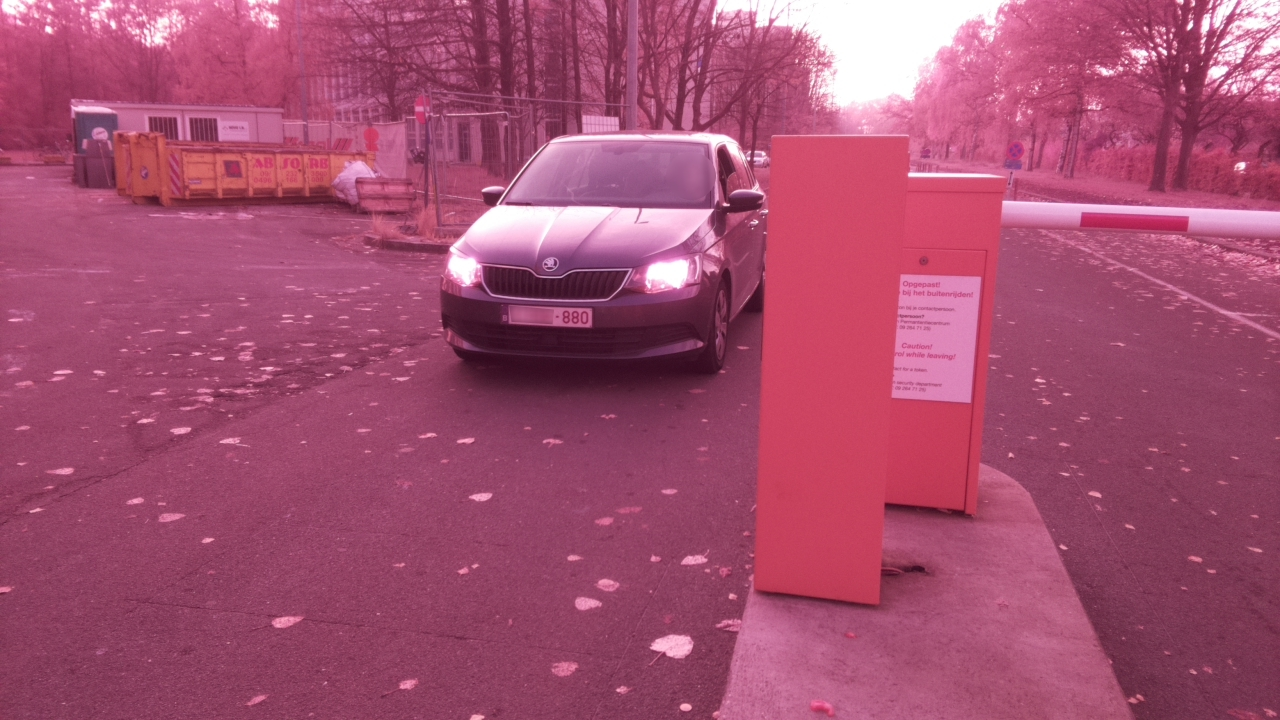
\includegraphics[width=0.5\linewidth]{img/res-galglaan/galg1.jpg}
	\caption{Niet-gedetecteerde nummerplaat aan Campus Sterre - Galglaan. Enkele karakters van de nummerplaat zijn onleesbaar gemaakt uit privacy van de bestuurder.}
	\label{foutiefgalglaan}
\end{figure}

\subsection{Campus Sterre - Uitgang De Pintelaan}
De uitgang op de Campus Sterre aan de De Pintelaan is de hoofduitgang van UGent Campus Sterre en was een uitdaging om correct te configureren. Deze is verbonden met drie straten die enkele grote parkings verbinden, bijgevolg wordt deze het meest gebruikt van alle uitgangen. Het is dan ook belangrijk dat hier een goede detectie is.

Door de vele verbindingen is het mogelijk om de parking op allerlei manieren te bereiken, deze zijn te zien op figuur \ref{fig:satellietdepintelaan}. Dit is op zich geen probleem, maar hierdoor moet de nummerplaatdetectie wel in een groot aantal oriëntaties werken.

Aangezien aan deze uitgang niet direct een optimale camerahoek gevonden was, worden in de volgende onderdelen de geteste camerahoeken beschreven tezamen met hun resultaten. Deze camerahoeken zijn aangeduid met cijfers in figuur \ref{fig:satellietdepintelaan}.

\begin{figure}[h!]
	\centering
	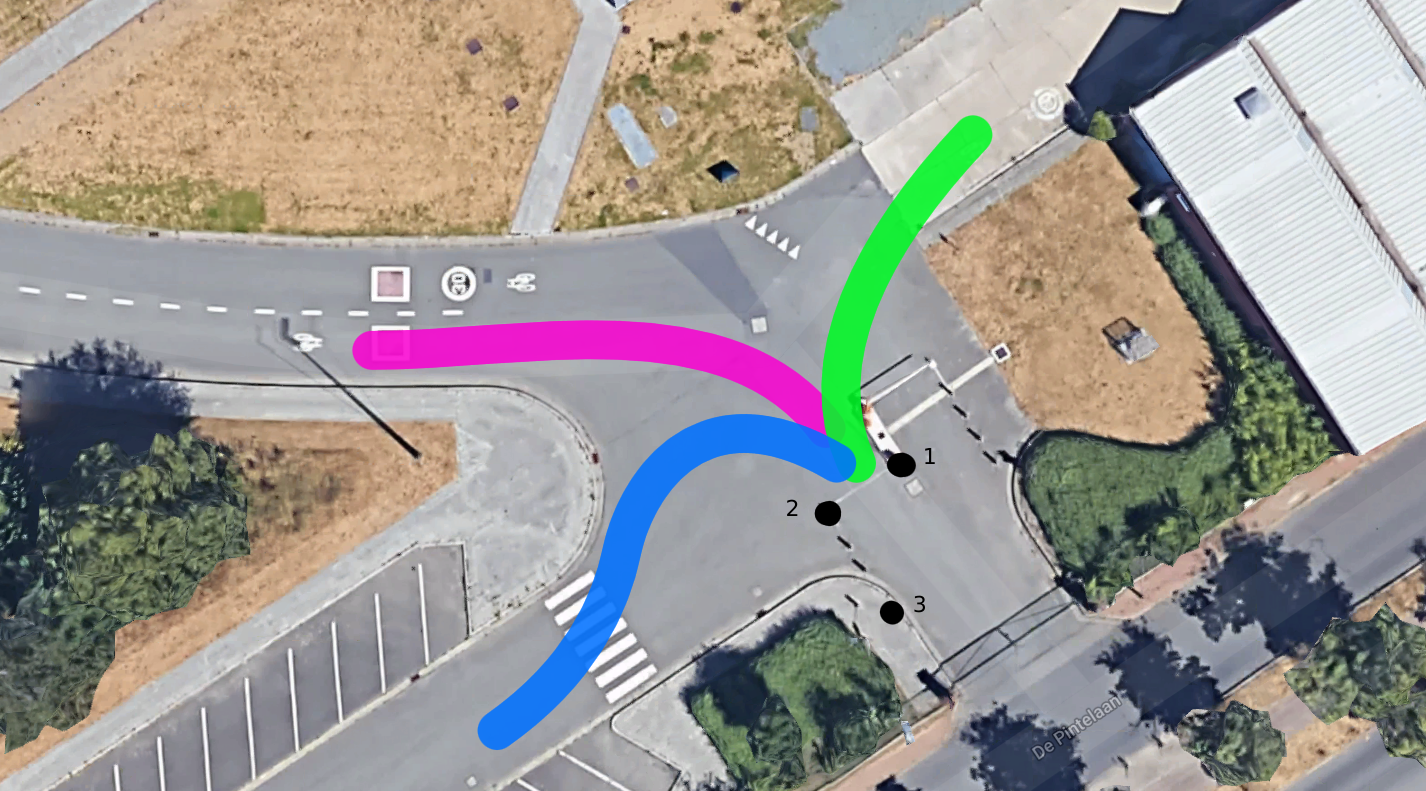
\includegraphics[width=\linewidth]{img/satellietdepintelaan.png}
	\caption{Satellietafbeelding van de Campus Sterre - Uitgang De Pintelaan met aangeduide routes en cameralocaties. \autocite{ugent2019google}}
	\label{fig:satellietdepintelaan}
\end{figure}

\subsubsection{Positie rechts van de hefboom}
In een eerste poging tot detectie werd de camera op de metalen constructie van de hefboom geplaatst, wat op de uitgang van de Galglaan al degelijke resultaten leverde. Spijtig genoeg was deze locatie duidelijk niet geschikt, de zon speelde een grote invloed op de afbeeldingen en ook de vele inrijrichtingen maakten dit moeilijk.

Deze plaatsing van de camera is aangeduid op afbeelding \ref{fig:satellietdepintelaan} als punt 1. Figuur \ref{fig:plaatsingdepintelaanorigineel} verduidelijkt de specifieke plaatsing van de camera zelf.

\begin{figure}[h!]
	\centering
	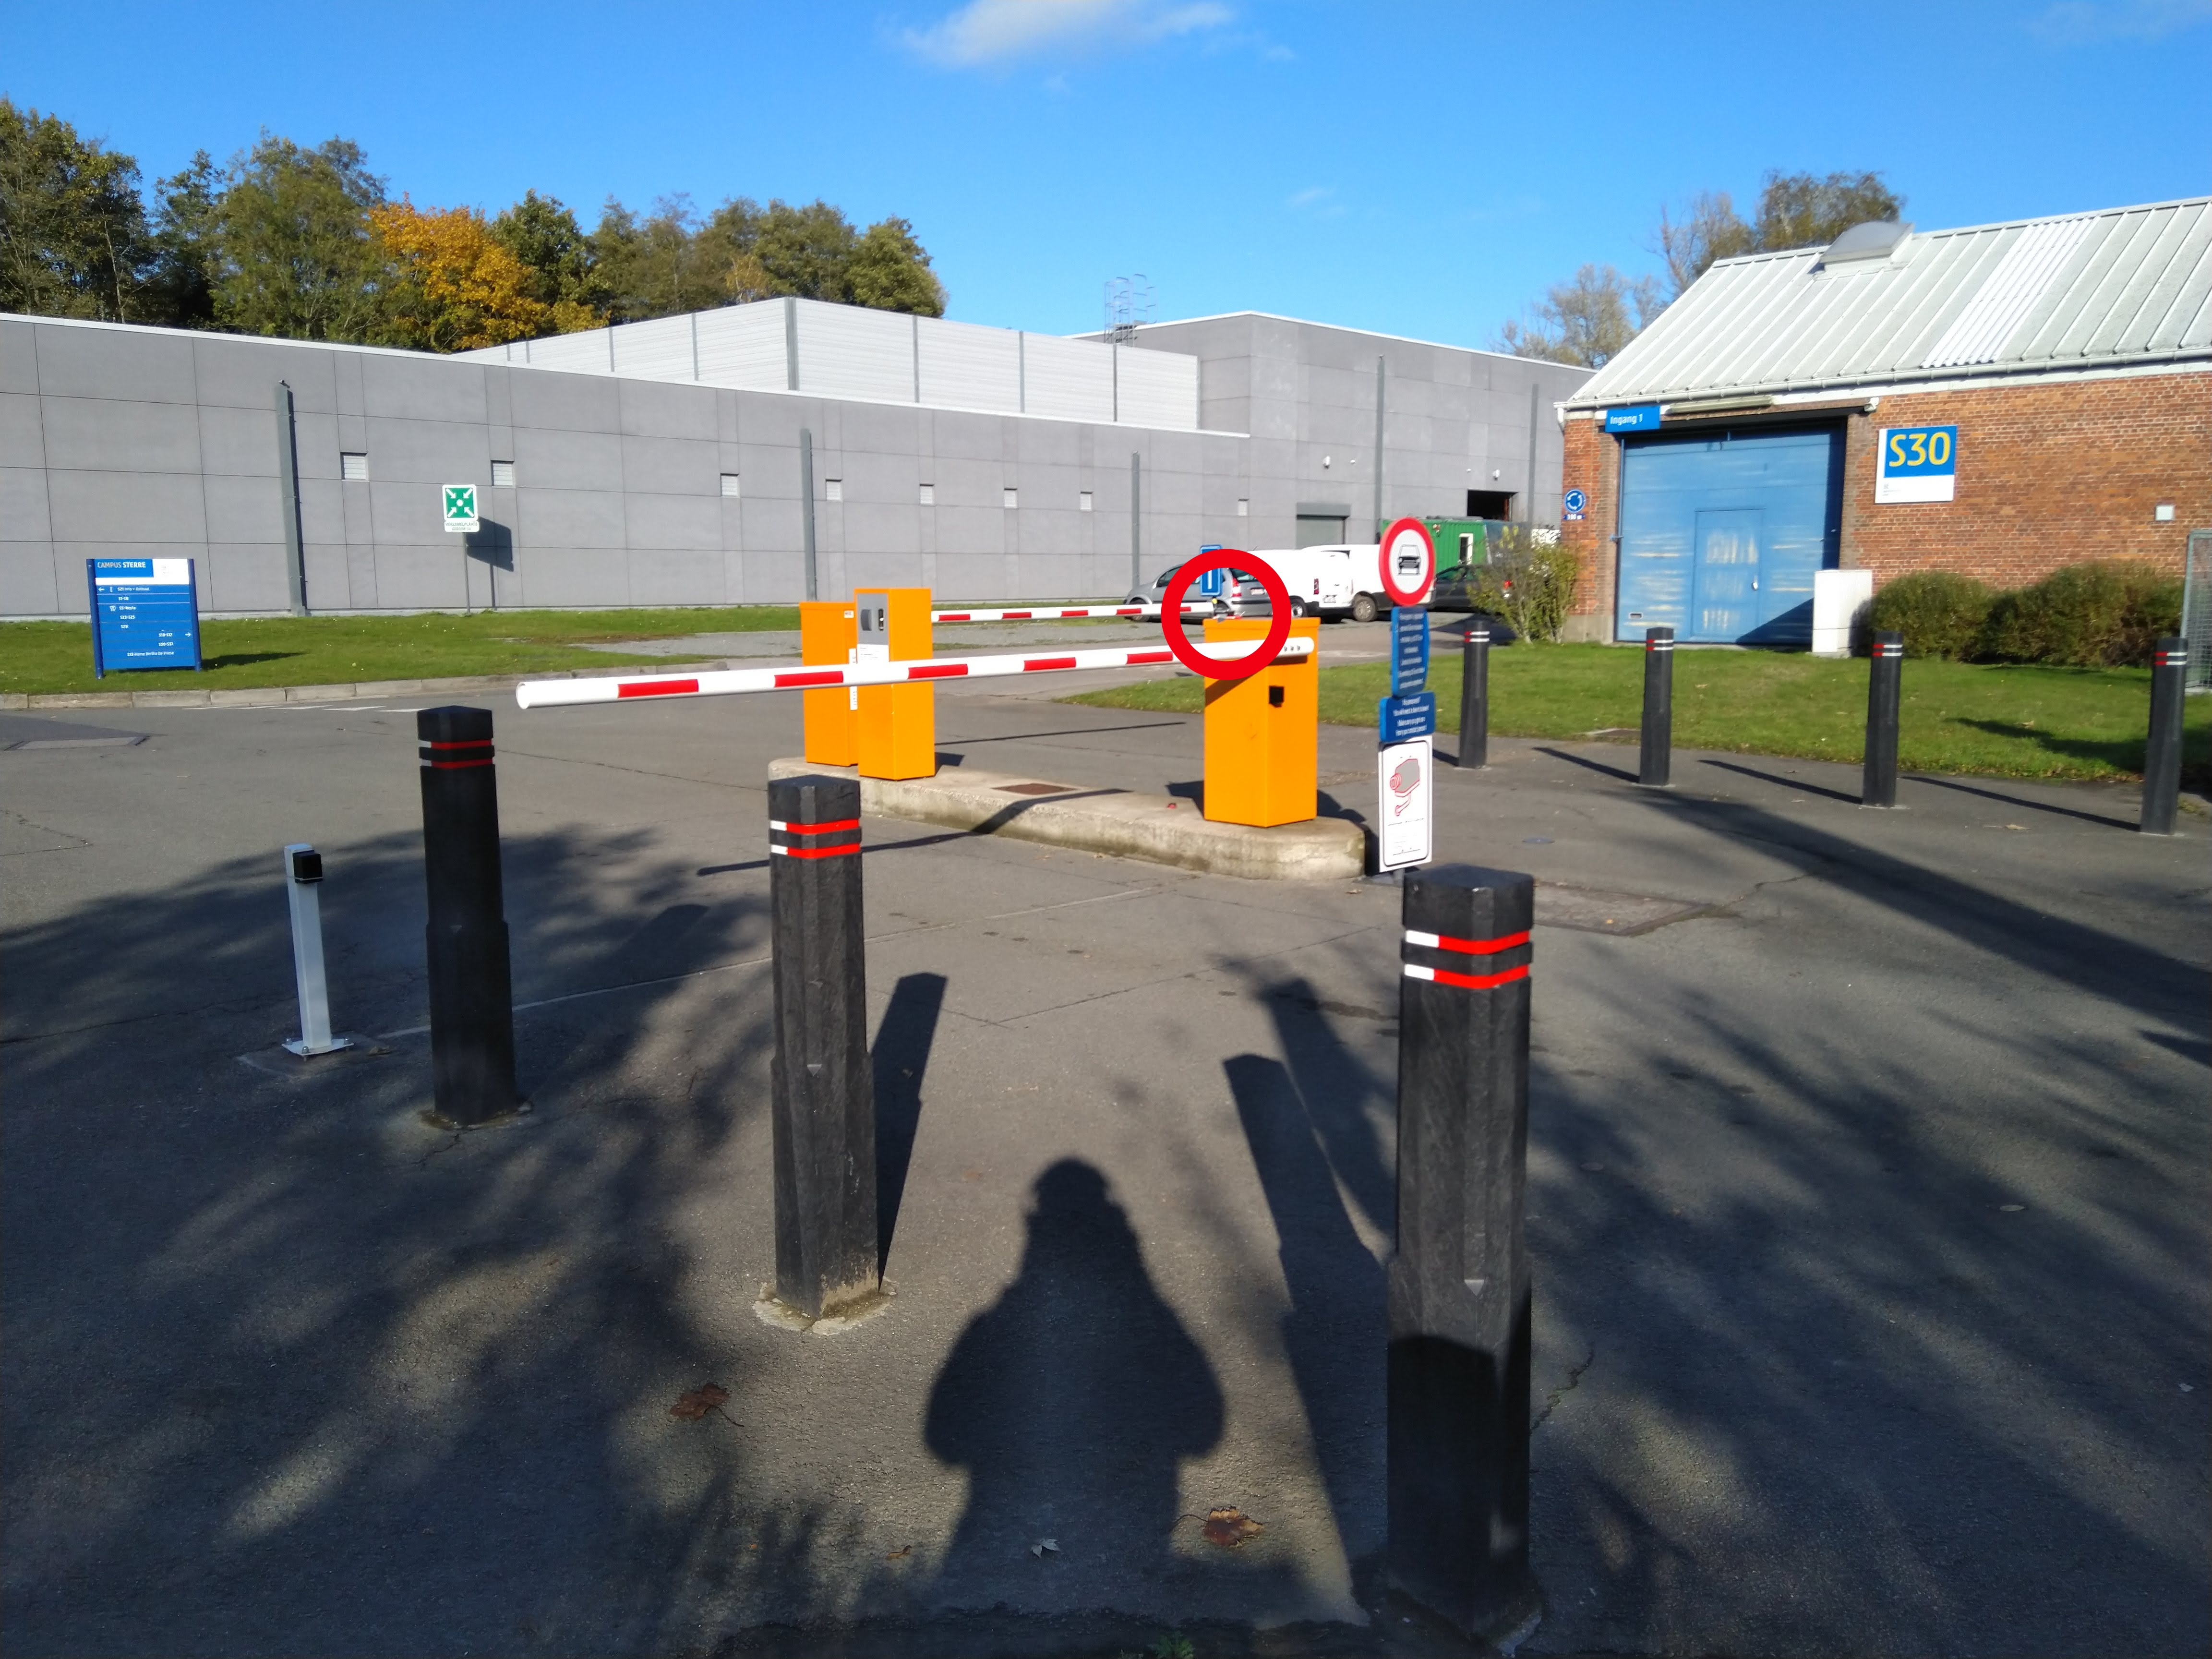
\includegraphics[width=0.8\linewidth]{img/depintelaanorigineel.jpg}
	\caption{Cameraplaatsing aan de rechterkant van de hefboom op Campus Sterre - De Pintelaan. De locatie van de camera is aangeduid met een rode cirkel. De uitrijrichting is van links naar rechts}
	\label{fig:plaatsingdepintelaanorigineel}
\end{figure}

\begin{table}[h!]
	\centering
	\begin{tabular}{l|l|l|l|l}
		\textbf{ANPR nauwkeurigheid: De Pintelaan, rechts} & Incorrect & Correct & Totaal & Ratio	\\ \hline
		Per individuele foto 	& 43	& 30	& 73 & 41.1\%\\
		Per auto				& 8	& 17 	& 25 & 68.0\%\\
	\end{tabular}
\caption{Resultaten van OpenALPR aan Campus Sterre - Uitgang Depintelaan, camerahoek 1.}
\label{tab:alprdepintelaan1}
\end{table}

De eerste resultaten aan deze uitgang waren niet denderend, indien 30\% van de bezoekers terug moeten keren om toch een token te halen doet nummerplaatdetectie meer kwaad dan goed. Na het inspecteren van de foutieve afbeelding werd duidelijk dat bij vele voertuigen 's middags een grote interferentie van het zonlicht hadden. Wanneer de zon hoog staat reflecteerde het zonlicht via de nummerplaat recht in de camera, wat het contrast van de tekst op de nummerplaat in grote mate verminderde en de detectie onmogelijk maakte. Hieruit kunnen we afleiden dat deze specifieke cameraplaatsing niet geschikt is voor de uitgang en een andere camerahoek gezocht moest worden. 

Een voorbeeld van deze interferentie is te zien op Figuur \ref{SterreZonlicht}. Deze afbeelding is niet bewerkt, de nummerplaat is gewoonweg helemaal niet zichtbaar door de reflectie van het zonlicht.
\begin{figure}[h!]
	\centering
	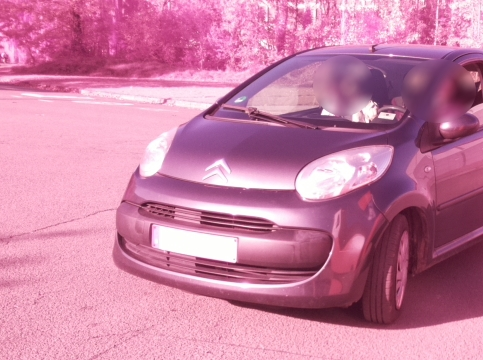
\includegraphics[width=0.8\linewidth]{img/sterre2zon.jpg}
	\caption{Interferentie van zonlicht op de parking van Campus Sterre - De Pintelaan, camerahoek 1.}
	\label{SterreZonlicht}
\end{figure}

\subsubsection{Positie links van de hefboom}
In een poging om de invloed van de zon tegen te gaan is geprobeerd om de camera aan de linkerkant van de slagboom te zetten, maar ook op deze positie maakte de zon de nummerplaten in vele gevallen minder leesbaar, bijkomend gaf de camerahoek zelf enkele nadelen. Door de vele inrijrichtingen van de auto, aangeduid op figuur \ref{fig:satellietdepintelaan}, waren een groot deel van de nummerplaten helemaal niet zichtbaar. Enkele voorbeelden hiervan zijn te zien in figuur \ref{fig:sterre-links}, Auto's die van links komen hun nummerplaten staan te schuin om soms zelfs duidelijk met het oog te kunnen lezen.

\begin{figure}[h!]
	\centering
	\begin{subfigure}[b]{0.4\linewidth}
		\includegraphics[width=\linewidth]{img/sterlinks/sterrelinks1.jpg}
	\end{subfigure}
	\begin{subfigure}[b]{0.4\linewidth}
		\includegraphics[width=\linewidth]{img/sterlinks/sterlinks2.jpg}
	\end{subfigure}
	\caption{Moeilijk te detecteren nummerplaten door scherpe camerahoek.}
	\label{fig:sterre-links}
\end{figure}

Hierdoor verkrijgen we volgende resultaten:
\begin{table}[h!]
	\centering
	\begin{tabular}{l|l|l|l|l}
		\textbf{ANPR nauwkeurigheid: De Pintelaan, links} & Totaal & Incorrect & Correct & Ratio	\\ \hline
		Per individuele foto 	& 50 & 31	& 19	& 38.0\%\\
		Per auto				& 17 & 8	& 9 	& 52.9\%\\
	\end{tabular}
\caption{Resultaten van OpenALPR aan Campus Sterre - Uitgang De Pintelaan, camerahoek 2.}
\label{tab:alprdepintelaan2}
\end{table}

Met een slechter resultaat dan de vorige positie en net meer dan de helft van de auto's correct te kunnen detecteren, kunnen we besluiten dat deze positie geen oplossing is.

\subsubsection{Positie achteraan de uitgang}
Als derde optie is er getest op de mogelijkheid om van een verdere locatie foto's te nemen aan de hand van een statief om de camera op een geschikte hoogte te houden. Dit is aangetoond op figuur \ref{plaatsingdepintelaan}. Door de camera naar achteren te zetten zorgen de inrijrichtingen voor geen problemen meer aangezien de wagens allemaal op dezelfde plaats kunnen gefotografeerd worden. Verder is er geen storing meer van het zonlicht omdat de camera hoog staat en naar omlaag is gericht.

Deze positie is een drie meter naar achteren van de linkerkant van de hefboom, dit zodat da invalshoek van de camera zo klein mogelijk blijft. De hoogte van de camera is 1,5 meter hoog, wat hoog genoeg was om de invloed van het zonlicht weg te werken.
\begin{figure}[h!]
	\centering
	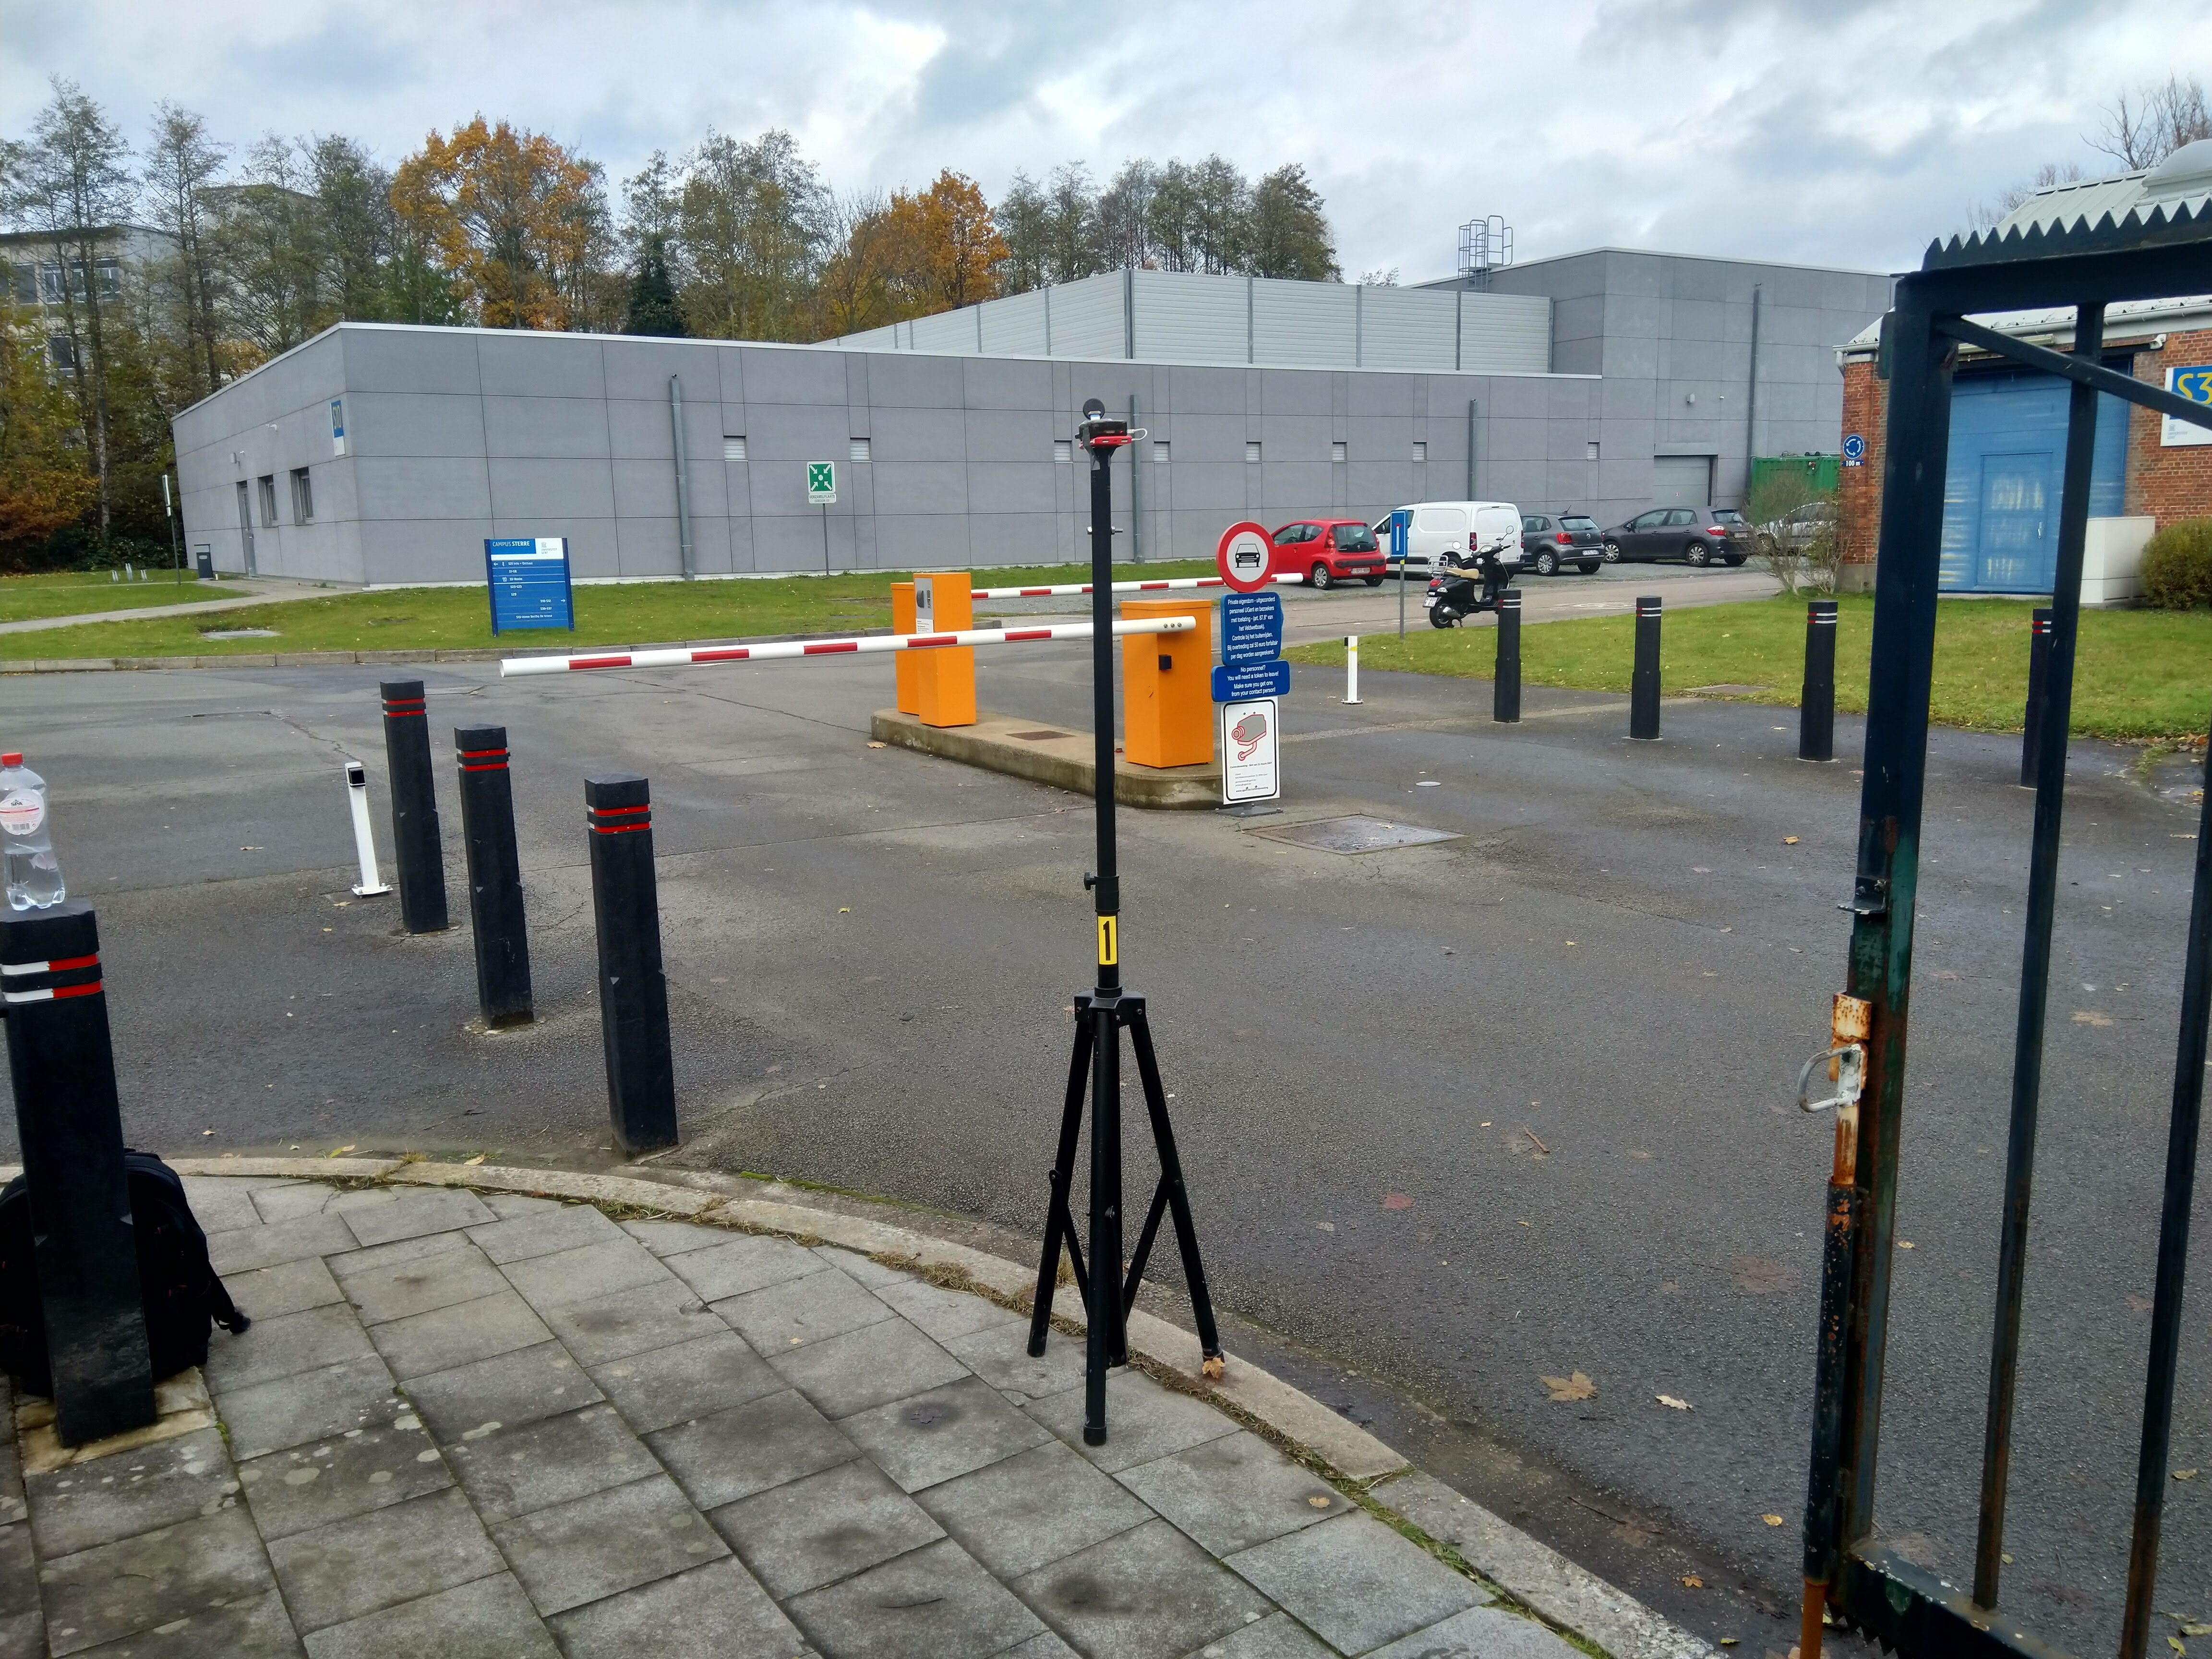
\includegraphics[width=0.8\linewidth]{img/depintelaanstatief.jpg}
	\caption{Cameraplaatsing met statief op Campus Sterre - De Pintelaan.}
	\label{plaatsingdepintelaan}
\end{figure}

Volgende resultaten zijn bekomen aan de uitgang:
\begin{table}[h!]
	\centering
	\begin{tabular}{l|l|l|l|l}
		\textbf{ANPR nauwkeurigheid: De Pintelaan, achteraan} & Totaal & Incorrect & Correct & Ratio	\\ \hline
		Per individuele foto 	& 75 & 35	& 40	& 53.3\%\\
		Per auto				& 24 & 6	& 18 	& 75.0\%\\
	\end{tabular}
\caption{Resultaten van OpenALPR aan Campus Sterre - Uitgang De Pintelaan, camerahoek 3.}
\label{tab:alprdepintelaan3}
\end{table}

Deze locatie is een verbetering t.o.v. de vorige posities. Allereerst staan alle auto's op dezelfde locatie ongeacht van inrijrichting. Dit maakt de configuratie van OpenALPR een pak aangenamer en betrouwbaarder.

Ondanks deze voordelen is de nauwkeurigheid niet hoog genoeg en zijn er toch 6 auto's die niet gedetecteerd zijn. Na deze na foto's te gaan is het duidelijk dat dit komt door de grote afstand en bijgevolg lagere resolutie van de nummerplaten. Een voorbeeld hiervan is te zien op figuur \ref{fig:lowressterre}.

Verder is één voertuig niet gedetecteerd niet door de lage resolutie maar door de hoogte van de slagboom, deze vrachtwagen zijn nummerplaat is te hoog aan het voertuig gemonteerd waardoor de slagboom ervoor staat op de foto. Dit is te zien in figuur \ref{fig:slagboomster}. Deze situatie is wellicht uitzonderlijk. Alle andere auto's hun nummerplaat zit ruim onder de slagboom.

\begin{figure}[h!]
	\centering
	\begin{subfigure}[b]{0.49\linewidth}
		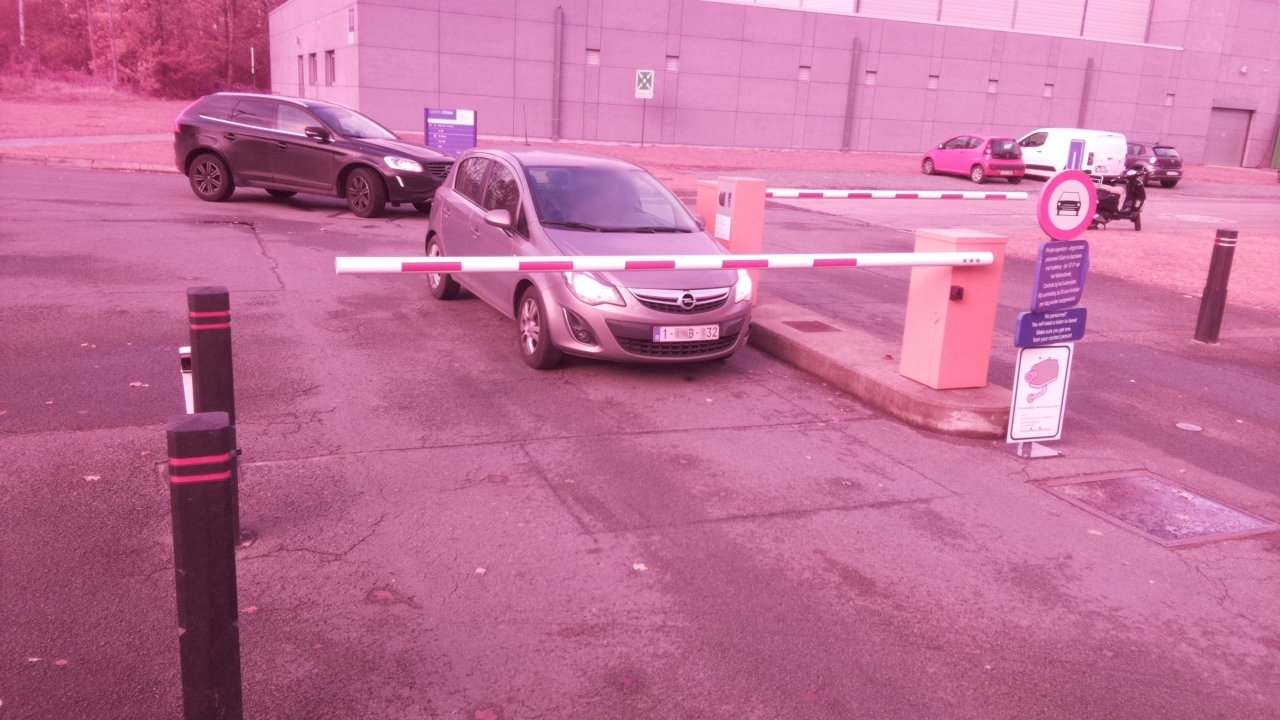
\includegraphics[width=\linewidth]{img/sterachter/sterachter1.jpg}
	\end{subfigure}
	\begin{subfigure}[b]{0.49\linewidth}
		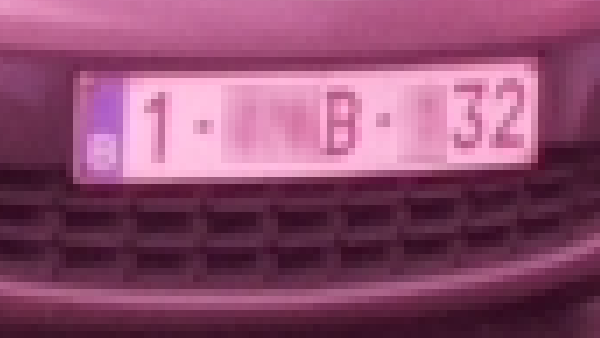
\includegraphics[width=\linewidth]{img/sterachter/sterachter2.png}
	\end{subfigure}
	\caption{Moeilijk te detecteren nummerplaten door een te lage resolutie. Enkele karakters zijn onduidelijk gemaakt uit privacy van de bestuurder.}
	\label{fig:lowressterre}
\end{figure}

\begin{figure}[h!]
	\centering
	\begin{subfigure}[b]{0.99\linewidth}
		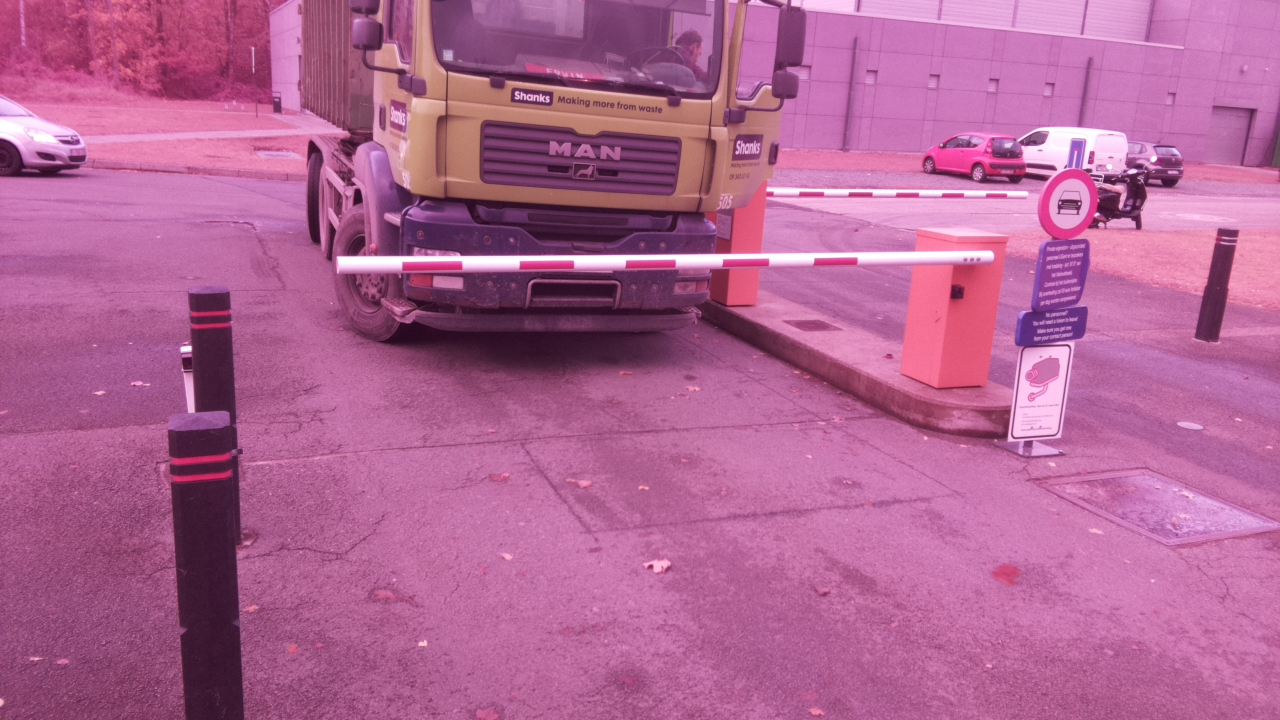
\includegraphics[width=\linewidth]{img/sterachter/sterachter3.jpg}
	\end{subfigure}
	\caption{Niet te detecteren nummerplaat omwille van slagboom die het zicht verhindert.}
	\label{fig:slagboomster}
\end{figure}

\subsubsection{Positie achteraan de uitgang - hoge resolutie}
Ten laatste is de steekproef op de vorige positie opnieuw uitgevoerd. De nauwkeurigheid van de PiNoIR camera biedt echter een veel hogere resolutie aan dan origineel ingesteld. Dit maakte het mogelijk om softwarematig in te zoomen op de foto's met een betere kwaliteit. In afbeelding \ref{fig:ressterrecomparison} is dit verschil van de foto's duidelijk te zien.

\begin{figure}[h!]
	\centering
	\begin{subfigure}[b]{0.49\linewidth}
		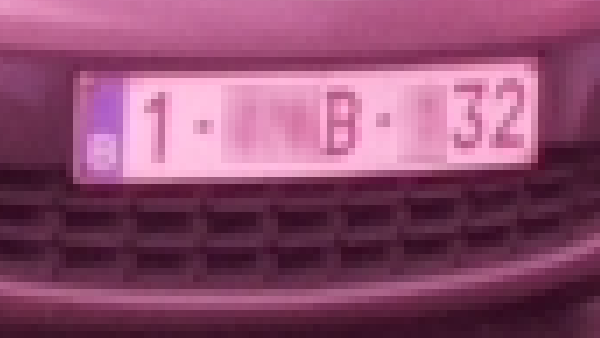
\includegraphics[width=\linewidth]{img/sterachter/sterachter2.png}
		\caption{Originele kwaliteit}
	\end{subfigure}
	\begin{subfigure}[b]{0.49\linewidth}
		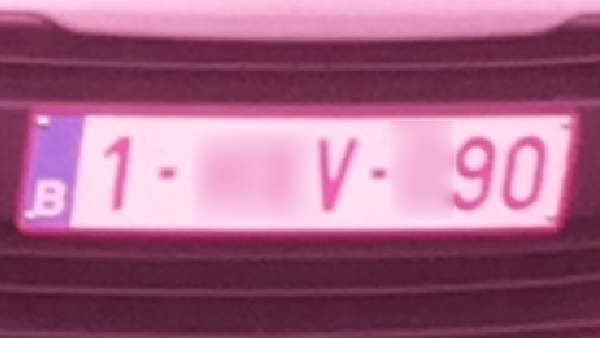
\includegraphics[width=\linewidth]{img/sterachter/hressmall2.png}
		\caption{Verhoogde kwaliteit}
	\end{subfigure}
	\caption{Verhoogde nauwkeurigheid door het inzoomen van de camera.}
	\label{fig:ressterrecomparison}
\end{figure}

Na de camera vervolgens opnieuw te kalibreren zijn volgende resultaten bekomen:
\begin{table}[h!]
	\centering
	\begin{tabular}{l|l|l|l|l}
		\textbf{ANPR nauwkeurigheid: De Pintelaan, achteraan} & Totaal & Incorrect & Correct & Ratio	\\ \hline
		Per individuele foto 	& 19 & 45	& 64	& 70.3\%\\
		Per auto				& 2 & 24	& 26 	& 92.0\%\\
	\end{tabular}
\caption{Resultaten van OpenALPR aan Campus Sterre - Uitgang De Pintelaan, camerahoek 3 met hogere resolutie.}
\label{tab:alprdepintelaan4}
\end{table}

Deze zijn een enorm verschil met het vorig resultaat van 75\% van de vorige foto's en bieden een haalbare oplossing voor de uitgang van de De Pintelaan.

\paragraph{Nadelen}
Indien een camera op deze locatie moet gezet worden zullen er enkele maatregelingen nodig zijn om de camera te plaatsen en van stroom te voorzien. Een paal zou in de straat moeten vastgezet worden en een reeks kabels voor stroom en data moeten naar de metalen constructie van de hefboom lopen. Dit vraagt een redelijke hoeveelheid meer werk en kosten dan een systeem dat op de behuizing zelf staat.

\paragraph{Verbeteringen}
De camera is niet direct te hoog geplaatst, dit was uit voorzorg dat de hefboom van de toegang het beeld van de nummerplaten overlapt. Na de foto's te analyseren bleek het toch dat er nog ruim veel plaats was om de camera hoger te zetten. Dit is een vereiste om mogelijke voorbijgangers te beletten van vandalisme. Er wordt verondersteld dat het verhogen van de camera geen direct negatieve invloed op de resultaten zal hebben, dit zolang de kalibratie opnieuw wordt uitgevoerd.

\subsection{Campus Coupure - Uitgang Kruisboogstraat}

De uitgang aan de Kruisboogstraat is de hoofduitgang van de Campus Coupure. Deze uitgang is zeer dichtbij gelegen met 3 van de 4 parkings van de campus, en heeft dus een redelijk hoog aantal auto's die deze gebruikt. Deze locatie is te zien in figuur \ref{fig:sat-kruisboog}, aangeduid met een rode cirkel. Een close-up van de uitgang is te zien in figuur \ref{fig:Kruisboog-uitgang}. 

\begin{figure}[h!]
	\centering
	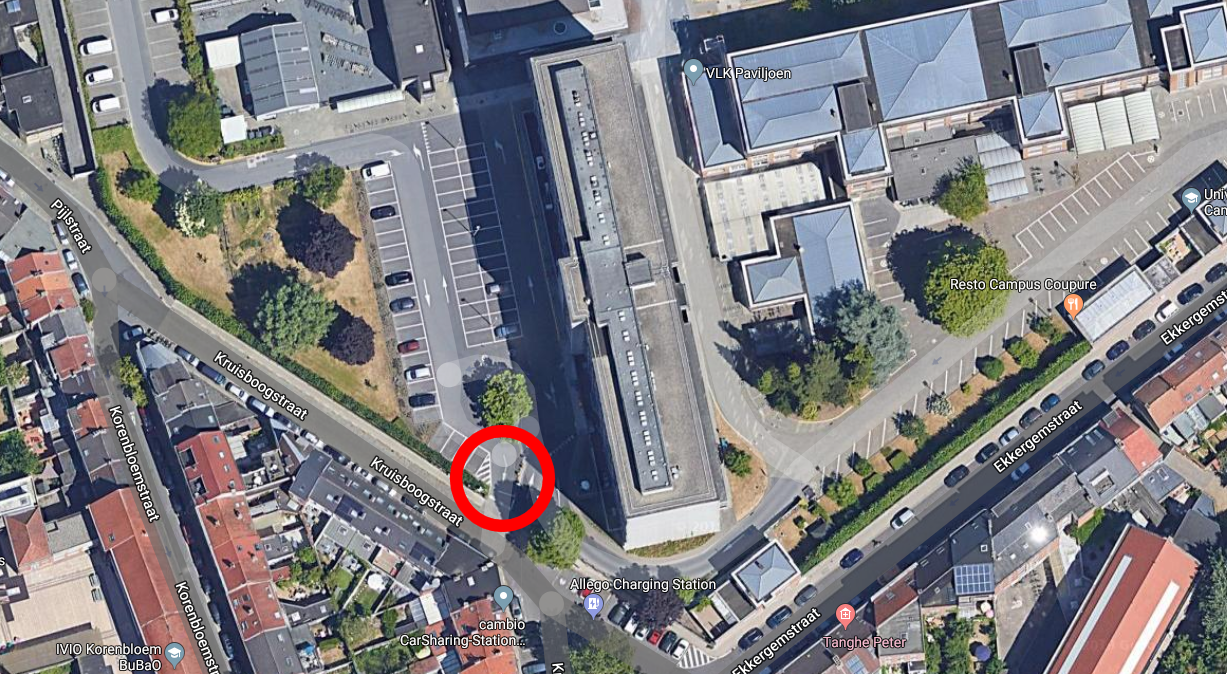
\includegraphics[width=\linewidth]{img/kruisboog/sateliet-kruisboog.jpg}
	\caption{Satellietafbeelding van de uitgang aan de Kruisboogstraat. De uitgang zelf is aangeduid met een rode cirkel. \autocite{ugent2019google}}
	\label{fig:sat-kruisboog}
\end{figure}

\begin{figure}[h!]
	\centering
	\includegraphics[width=0.9\linewidth]{img/kruisboog/kruisboog-uitgang.jpg}
	\caption{Close-up foto van de uitgang aan de Kruisboogstraat. De locatie van de camera is aangeduid met een rode cirkel.}
	\label{fig:Kruisboog-uitgang}
\end{figure}

Er werd gekozen om de camera op de metalen constructie van de hefboom te plaatsen aangezien deze een brede kijk geeft op alle mogelijke inrijrichtingen, wat te zien is in figuur \ref{fig:Kruisboog}, maar ook omdat deze bij een werkelijke implementatie gemakkelijk te monteren zou zijn. Dit omdat enkele bekabelingen reeds aanwezig is in de montage van de hefboom.

\begin{figure}[h!]
	\centering
	\includegraphics[width=0.7\linewidth]{img/kruisboog/kruisboog.jpg}
	\caption{Voorbeeld van een ANPR-foto aan de uitgang Kruisboogstraat. Enkele tekens van de nummerplaat zijn onleesbaar gemaakt uit privacy van de bestuurder.}
	\label{fig:Kruisboog}
\end{figure}

\subsubsection{Resultaten}

Met deze positie en camerahoek zijn de volgende resultaten bekomen:

\begin{table}[h!]
	\centering
	\begin{tabular}{l|l|l|l|l}
		\textbf{ANPR nauwkeurigheid: Kruisboogstraat} & Incorrect & Correct & Totaal & Ratio	\\ \hline
		Per individuele foto 	& 16 & 52	& 68	& 76.5\%\\
		Per auto				& 1 & 25	& 26 	& 96.15\%\\
	\end{tabular}
	\caption{Resultaten van OpenALPR aan Campus Sterre - Uitgang Kruisboogstraat.}
	\label{ResultatenKruisboog}
\end{table}

De behaalde marge van 96.15\% is boven de gewenste nauwkeurigheid van 95\%. Waardoor besloten kan worden dat nummerplaatdetectie een haalbare technologie is aan de uitgang aan de Kruisboogstraat. Deze resultaten gelden enkel voor detectie overdag, zonder moeilijke weersomstandigheden.

\subsubsection{Fouten}
Op 1 auto na zijn alle auto's correct geïdentificeerd. De incorrecte afbeeldingen hebben geen merkwaardige verschillen van de andere afbeeldingen waardoor de juistheid lager zou liggen. We kunnen hieruit dus veronderstellen dat deze fout komt door de nauwkeurigheid van OpenALPR zelf. Mogelijks zou het verhogen van de resolutie van de camera een verbetering hebben op deze resultaten.

\begin{figure}[h!]
	\centering
	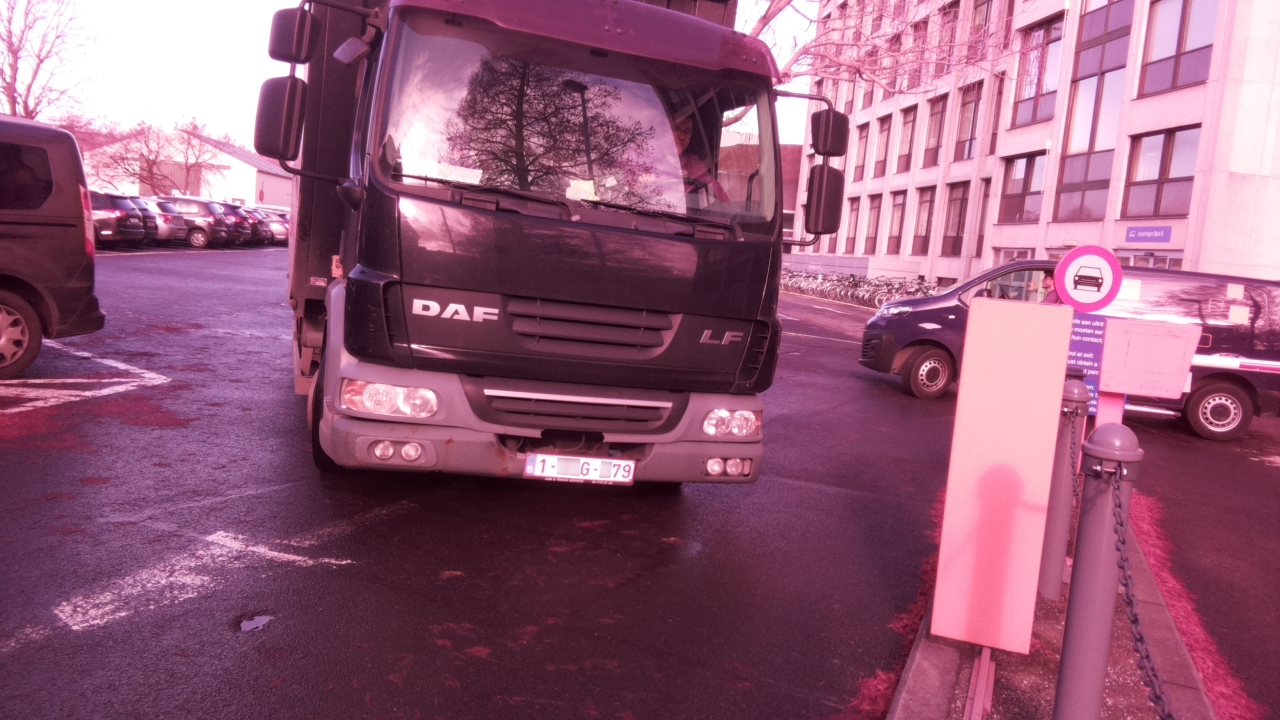
\includegraphics[width=0.8\linewidth]{img/kruisboog/kruisboog-incorrect.jpg}
	\caption{Een niet-geïdentificeerd voertuig aan de uitgang Kruisboogstraat. Enkele tekens van de nummerplaat zijn onleesbaar gemaakt uit privacy van de bestuurder.}
	\label{fig:kruisboog-incorrect}
\end{figure}

\subsection{Campus Coupure - Uitgang Coupure Links}
De uitgang aan de Coupure Links, afgebeeld in figuur \ref{fig:coupure-links}, had niet genoeg doorrijdende auto's om een degelijke steekproef te nemen, of een correcte cameraconfiguratie te vinden. Op een tijdsduur van 2u waren er in totaal 4 auto's gepasseerd. Het was niet mogelijk om de tijd te voorzien om genoeg foto's te verzamelen of om een opstelling te maken die achtergelaten kon worden. Hierdoor is deze uitgang niet verwerkt in dit onderzoek.

\begin{figure}[h!]
	\centering
	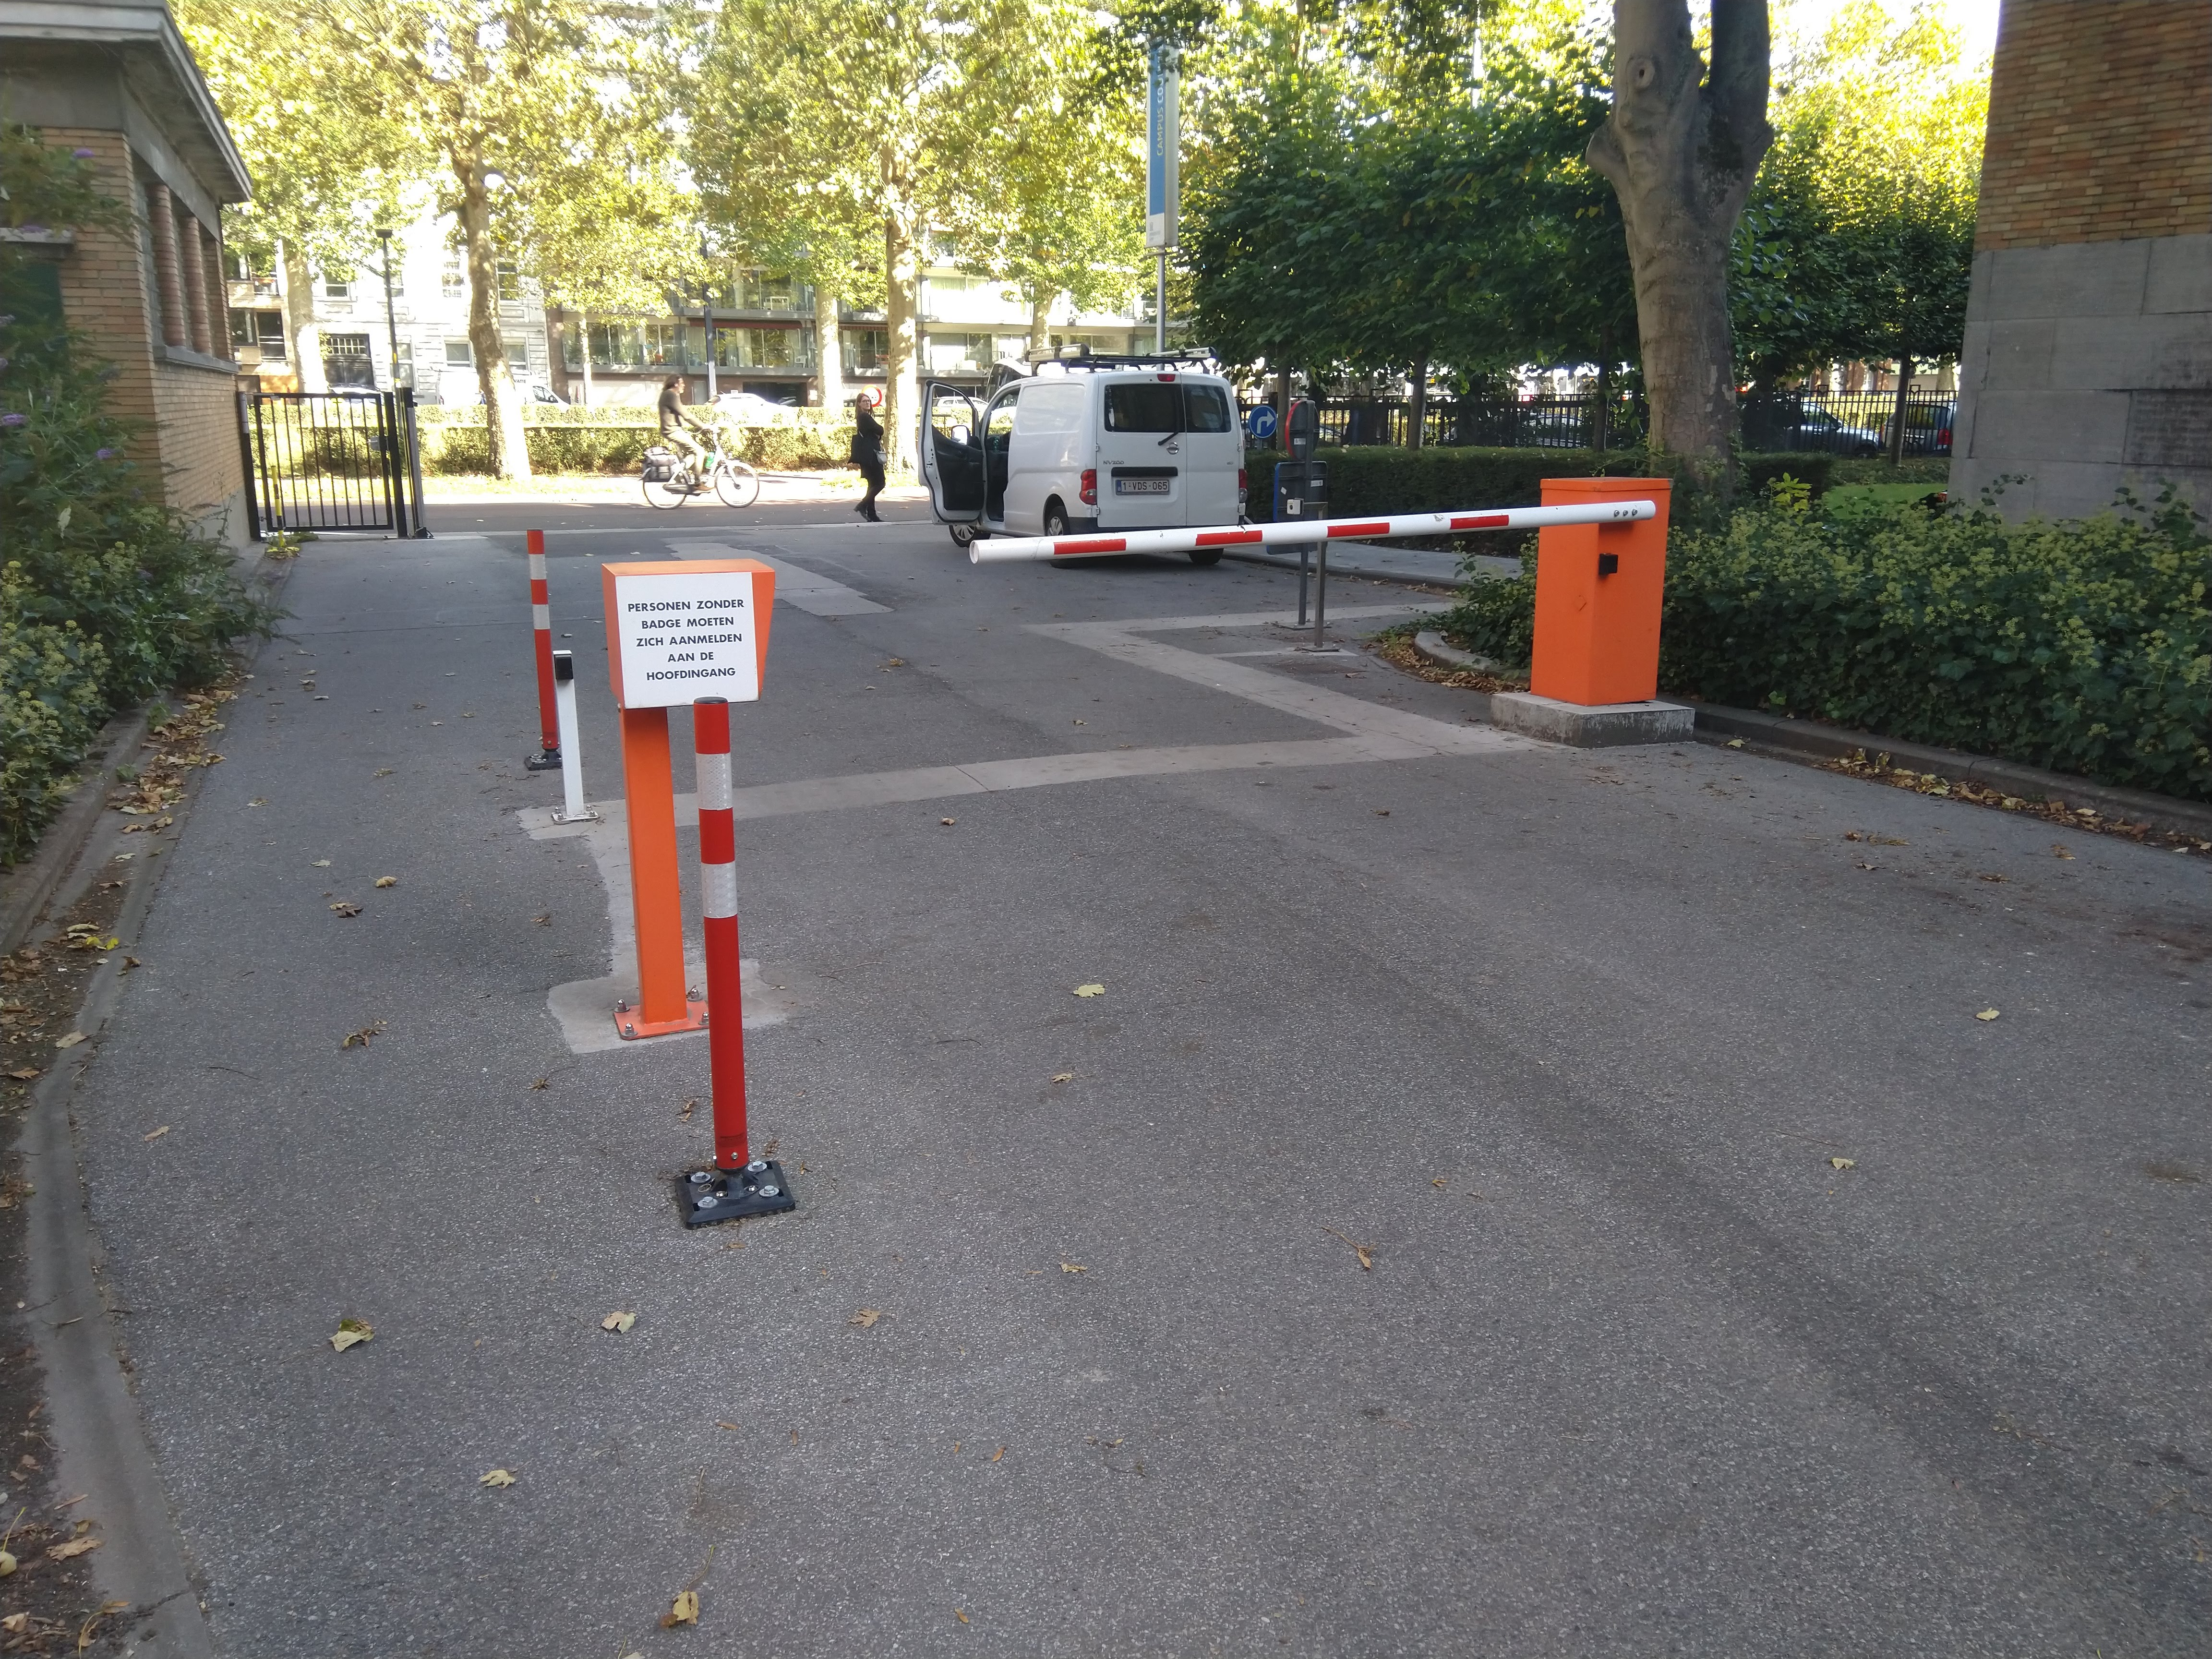
\includegraphics[width=0.8\linewidth]{img/coupure-links/coupure-links.jpg}
	\caption{Foto van de uitgang Coupure Links.}
	\label{fig:coupure-links}
\end{figure}

\section{Algemene resultaten}
%In het donker is de interferentie van de koplampen niet te groot, maar de algemene donkerheid van de omgeving zorgt ervoor dat de raspberry pi zijn shutter te lang openhoudt en dat de afbeeldingen enorm donker blijken. Het is dus vereist om extra infraroodbelichting bij te plaatsen.
%\begin{figure}[h!]
%	\centering
%	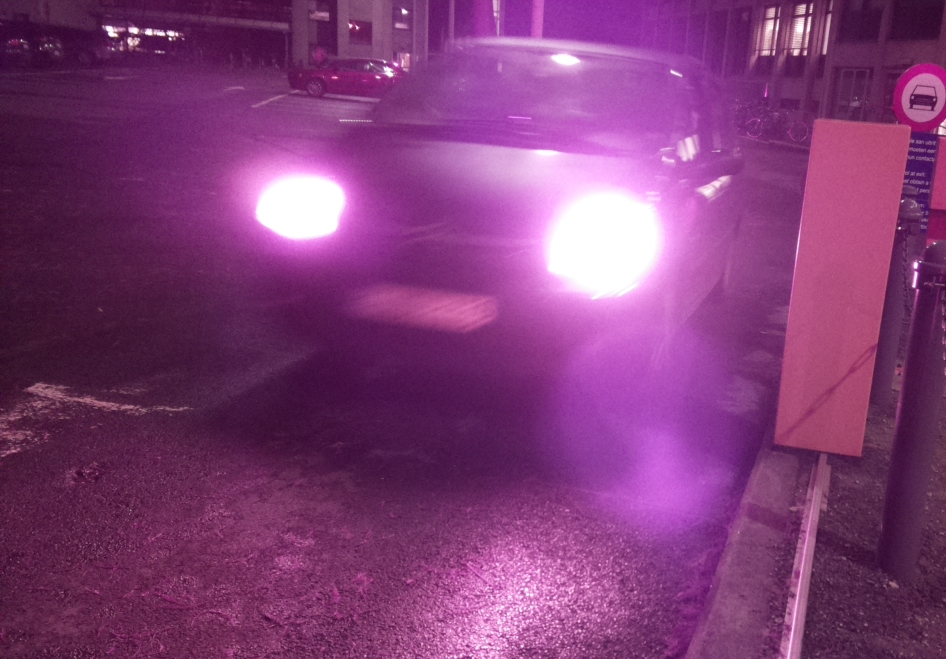
\includegraphics[width=0.5\linewidth]{img/nacht-coupure.jpg}
%	\caption{Onnauwkeurige foto's door een tekort aan licht.}
%	\label{SterreDonker}
%\end{figure}

\begin{table}[h!]
	\centering
	\begin{tabular}{l|l|l|l|l}
		\textbf{Resultaten per individuele foto}	& \textbf{Incorrect}	& \textbf{Correct} & \textbf{Aantal foto's} & \textbf{Ratio} \\ \hline
		Campus Coupure - Uitgang Kruisboogstraat & 16 & 52 & 68 & 76.5\% \\
		Campus Sterre - Uitgang Galglaan 		 & 13 & 49 & 62 & 79.0\%\\
		Campus Sterre - Uitgang De Pintelaan	 & 19 & 45 & 64 & 70.3\%\\ \hline
		Totaal 									 & 48 & 146 & 194 & 75.3\%
	\end{tabular}
	\caption{Resultaten van nummerplaatdetectie per foto.}
	\label{tab:perpic}
\end{table}

\begin{table}[h!]
	\centering
	\begin{tabular}{l|l|l|l|l}
		\textbf{Resultaten per auto} & \textbf{Incorrect}	& \textbf{Correct} & \textbf{Aantal auto's} & \textbf{Ratio} \\ \hline
		Campus Coupure - Uitgang Kruisboogstraat& 1 & 25  & 26 & 96.15\% \\
		Campus Sterre - Uitgang Galglaan		& 1 & 22  & 23 & 95.7\%\\
		Campus Sterre - Uitgang De Pintelaan	& 2 & 24  & 26 & 92.0\%\\ \hline
		Totaal 									& 4 & 71 & 75 & 94.7\%
	\end{tabular}
	\caption{Resultaten van nummerplaatdetectie per auto.}
	\label{tab:percar}
\end{table}

Er werd in dit onderzoek vertrokken met de hypothese dat in een steekproef met nummerplaatdetectie een nauwkeurigheid boven de 95\% behaald kon worden. Dit resultaat was dan ook bevestigd bij twee van de drie beschreven uitgangen in tabel \ref{tab:percar}.

Een goedkope implementatie voor nummerplaatdetectie is dan ook in zekere mate mogelijk. Op twee van de drie geteste uitgangen is het mogelijk om de camera's op de metalen constructie naast de hefbomen te plaatsen en degelijke resultaten te behalen. Enkel op de uitgang aan de De Pintelaan is er noodzaak aan een uitgebreidere implementatie om de camera te kunnen monteren.

Aan de De Pintelaan voldeed de positie op de metalen constructie niet om degelijke resultaten te behalen en was een verhogen en verplaatsing noodzakelijk. Om nummerplaatdetectie aan deze uitgang te voorzien zou er dus een extra investering gemaakt moeten worden in het opzetten van een verhoging voor de camera en het leggen van kabels naar deze positie.

In het algemeen zijn de resultaten van dit onderzoek veelbelovend, maar kan er niet aangenomen worden dat deze gelden voor de volledige populatie. Toch stellen deze zeker de weg open naar breder onderzoek.

%\section{Uitbreidingen}
%Locatie van de sensor kan mss in het midden van balk \autocite{buhus2016automatic}.